\documentclass[pdflatex,sn-mathphys-num]{sn-jnl}% Math and Physical Sciences Numbered Reference Style

\usepackage{graphicx}%
\usepackage{multirow}%
\usepackage{amsmath,amssymb,amsfonts}%
\usepackage{amsthm}%
\usepackage{mathrsfs}%
\usepackage[title]{appendix}%
\usepackage{xcolor}%
\usepackage{textcomp}%
\usepackage{manyfoot}%
\usepackage{booktabs}%
\usepackage{algorithm}%
\usepackage{algorithmicx}%
\usepackage{algpseudocode}%
\usepackage{listings}%
\usepackage{bm}

\usepackage{bbding}     % \FiveStarOpen, \FiveStar (filled)
\usepackage{wasysym}    % \ocircle, \Square, etc.

\usepackage{tikz}
\usetikzlibrary{shapes.geometric}
\newcommand{\mReactant}{\tikz\draw[fill=white] (0,0) circle (1.1pt);}
\newcommand{\mTS}{\tikz\node[star, star points=5, draw, fill=white, inner sep=0.8pt]{};}
\newcommand{\mProduct}{\tikz\node[regular polygon, regular polygon sides=3, draw, fill=white, inner sep=0.6pt]{};}

\theoremstyle{thmstyleone}%
\newtheorem{theorem}{Theorem}%  meant for continuous numbers
\newtheorem{proposition}[theorem]{Proposition}% 
\theoremstyle{thmstyletwo}%
\newtheorem{example}{Example}%
\newtheorem{remark}{Remark}%
\theoremstyle{thmstylethree}%
\newtheorem{definition}{Definition}%

\raggedbottom

\usepackage{lineno}
\linenumbers

\begin{document}

\title[HIP: Hessian Interatomic Potentials]{Shoot from the HIP: Hessian Interatomic Potentials without derivatives}

%%=============================================================%%
%% Authors
%%=============================================================%%

\author[1,2,7,]{\fnm{Andreas} \sur{Burger}}
% \equalcont{These authors contributed equally to this work.}
% c@andreas-burger.com

\author[1,2,7,]{\fnm{Luca} \sur{Thiede}}
% \equalcont{These authors contributed equally to this work.}

\author[3,6]{\fnm{Nikolaj} \sur{Rønne}}

\author[1,2]{\fnm{Nandita} \sur{Vijaykumar}}

\author[1,4]{\fnm{Varinia} \sur{Bernales}}

\author[3,6]{\fnm{Tejs} \sur{Vegge}}

\author[3,6]{\fnm{Arghya} \sur{Bhowmik}}

\author*[1,2,4,5,7]{\fnm{Alán} \sur{Aspuru-Guzik}}\email{alan@aspuru.com}

%%=============================================================%%
%% Affiliations
%%=============================================================%%

% Address CS Dept
\affil[1]{\orgdiv{Department of Computer Science}, \orgname{University of Toronto}, \orgaddress{\street{40 St. George St.}, \city{Toronto}, \state{ON}, \postcode{M5S 2E4}, \country{Canada}}}

% Vector
\affil[2]{\orgname{Vector Institute for Artificial Intelligence}, \orgaddress{\street{W1140-108 College St., Schwartz Reisman Innovation Campus}, \city{Toronto}, \state{ON}, \postcode{M5G 0C6}, \country{Canada}}}

% DTU Address
\affil[3]{\orgdiv{Department of Energy Conversion and Storage}, \orgname{Danmarks Tekniske Universitet}, \orgaddress{\street{Anker Engelunds Vej 101}, \postcode{2800}, \city{Kongens Lyngby}, \country{Denmark}}}

% Address Acceleration Consortium
\affil[4]{\orgname{Acceleration Consortium}, \orgaddress{\street{700 University Ave.}, \city{Toronto}, \state{ON}, \postcode{M7A 2S4}, \country{Canada}}}

% Address Chemistry
\affil[5]{\orgdiv{Department of Chemistry}, \orgname{University of Toronto}, \orgaddress{\street{80 St. George St.}, \city{Toronto}, \state{ON}, \postcode{M5S 3H6}, \country{Canada}}}

% Address Capex
\affil[6]{\orgname{CAPeX Pioneer Center for Accelerating P2X Materials Discovery}, \orgaddress{\street{Anker Engelunds Vej 1, Bygning 101A}, \postcode{2800}, \city{Kgs. Lyngby}, \country{Denmark}}}

% Address NVIDIA
\affil[7]{\orgname{NVIDIA}, \orgaddress{\street{431 King St. W \#6th}, \city{Toronto}, \state{ON}, \postcode{M5V 1K4}, \country{Canada}}}

%%==================================%%
%% Abstract %%
%%==================================%%

\abstract{
Molecular Hessians, the second derivatives of the potential energy, are fundamental to many workflows in computational chemistry. Usually, accurate Hessians are computationally expensive to calculate and scale poorly with system size, whether computed using quantum chemistry methods or machine-learning interatomic potentials (MLIPs). In this work, we introduce Hessian interatomic potentials (HIPs), a deep learning model that directly predicts Hessians without relying on automatic differentiation or finite differences. To do so, we construct SE(3)-equivariant, symmetric Hessians from irreducible representation (irrep) features up to degree $l$=2, computed by a graph neural network. HIP Hessians are one to two orders of magnitude faster, more accurate, more memory efficient, easier to train, and exhibit favourable scaling with system size. We validate our predictions across a wide range of downstream tasks, demonstrating consistently superior performance in transition state search, geometry optimization, zero-point energy corrections, and vibrational analysis. We open-source the HIP code and model weights.
}

\keywords{Hessian, Machine Learning Interatomic Potentials, Equivariance, Transition States}

\maketitle

\section{Introduction}\label{sec1}

Molecular simulation is a cornerstone of material discovery and molecular design. While the prediction of energy and forces is often sufficient for structural dynamics, advanced computational chemistry workflows often depend on the molecular Hessian\citep{qu2016,huang2018}. By describing the local curvature of the potential energy surface (PES), the Hessian is foundational to many computational workflows. Second-order geometry optimization rely on the curvature information to rapidly and reliably converge to equilibrium structures\cite{schlegel2011}. Transition state (TS) searches and extrema classification depend on the Hessian to correctly identify saddle points and reaction barriers, which are essential for parameterizing reaction rates and microkinetic models for longer time and length scale simulations\cite{andersen2019}. Furthermore, mode-following transition state search methods directly leverage the curvature information to locate the transition states\cite{henkelman1999}. Finally, vibrational analysis use Hessian eigenvalues to compute zero-point energy (ZPE) corrections and thermodynamic free energies bridging the gap from static molecules to non-zero temperature observables\cite{grimme2012}. 
%Beyond energy and forces, workflows such as second-order geometry optimization, transition-state search, and vibrational analysis rely on Hessians \citep{qu2016,huang2018}. 


For a molecule with $N$ atoms, the Hessian is a $3N \times 3N$ matrix, where each entry requires a mixed second-order derivative of the electronic energy with respect to two nuclear coordinates. Despite their broad utility, Hessian calculations represent a significant computational bottleneck.
%\begin{equation}
%\mathbf{H}_{IJ}^{\alpha,\beta}\;=\;\frac{\partial^2 E}{\partial %\mathbf{R}_I^{\alpha}\,\partial \mathbf{R}_J^{\beta}}
%\end{equation}
%ewith $I,J=1,\dots,N$ indexing atoms, and $\alpha,\beta\in\{x,y,z\}$ indexing the cartesian $x,y$ and $z$ components of the atom positions $\mathbf{R}$. \\
Traditional approaches to obtain the Hessian rely either on analytic second derivatives or on numerical differentiation of gradients, both of which are very expensive, and analytical Hessians in particular are often so complicated to implement that they are not widely supported for all methods \citep{jorgensen1983,handy1984,komornicki1993}.

Most computational chemistry calculations are carried out with Kohn-Sham density functional theory \citep{kohn1965} (DFT), due to its balance of computational cost and accuracy \citep{bursch2022}.
However, the $O(N^4)$ scaling of hybrid DFT with system size remains expensive, which has spurred the development of machine-learning interatomic potentials (MLIPs). MLIPs promise to deliver near-DFT accuracy at a fraction of the cost while incorporating symmetries, thereby drastically reducing the need for extensive training data \citep{schutt2018,thomas2018,gasteiger2021,schutt2021,batatia2022,batzner2022}.
While recent work demonstrates that automatic differentiation (AD) can successfully recover the Hessian \citep{yang2024, yuan2024, gonnheimer2025, rodriguez2025, williams2025, cui2025horm}, this approach faces two significant limitations. First, high accuracy of the energy and forces does not guarantee comparably accurate second derivatives; much like training on force labels is needed to achieve accurate force predictions \cite{christensen2020forces}, explicit Hessian training labels are required for reliable AD Hessians \citep{zhao2025, cui2025horm}. 
Second, these AD Hessians introduce high computational costs, with an extra factor of $\sim{}3N$ during training and inference \citep{yuan2024,gonnheimer2025,rodriguez2025,williams2025,cui2025horm}. 
Rodriguez et al. ~\cite{rodriguez2025} in particular showed that including the Hessian in the loss improves data efficiency and extrapolation of energy and force predictions but is limited by approximately 25 times longer training times, which make AD Hessians prohibitive to train. The same principle extends to learned exchange-correlation functionals, where supervising energy derivatives substantially improves accuracy \citep{eberhard2026derivative}.
MLIPs can also be used to obtain Hessians with finite differences \citep{gonnheimer2025, fu2025}, an approach which requires less memory but $6N$ forward passes and also requires specialized data collection schemes to be accurate \cite{wander2025accessing}.\\

In this work, we introduce \textbf{HIP}: \textbf{H}essian \textbf{I}nteratomic \textbf{P}otentials. HIPs predict the Hessian directly, to eliminate the need for finite differences, coupled-perturbed equation solvers, or automatic differentiation. By building on SE(3)-equivariant neural networks, HIP construct the full $3N \times 3N$ matrix Hessian at a fraction of the cost of traditional methods. We demonstrate that HIP accelerates predictions 10-70$\times$ and reduces peak memory by a factor of 2-3 compared to AD, while maintaining a highly favourable $O(N)$ scaling with the number of atoms. Furthermore, HIP achieves superior predictive accuracy, halving the mean absolute error compared to AD. We validate the practical utility of HIP across several critical downstream applications, demonstrating consistently superior performance in second-order geometry optimization, ZPE corrections, TS searches and frequency analysis for extrema classification.

%, we demonstrate how HIP can predict Hessians at a fraction of the computational cost of traditional methods. 

%A key observation is that one can construct the Hessian from spherical-harmonic features of the atom nodes and the messages between atoms, satisfying equivariance and symmetry constraints by design. 
%In practice, HIP is not only faster but also more accurate than AD, enabling a variety of critical tasks in molecular simulations.\\

%We show that, compared to AD, the HIP predicted Hessians are at least 10-70$\times$ faster and consume 2-3$\times$ less peak memory on small molecules with 5-30 atoms, while scaling better by an order of $O(N)$ in the number of compute passes through the neural network.
%The predicted Hessians are furthermore accurate on the Hessian dataset for Optimizing Reactive MLIP (HORM) \cite{cui2025horm}, with 2$\times$ lower Hessian mean absolute error (MAE), 3.5$\times$ lower eigenvalue MAE, and 1.5$\times$ higher eigenvector cosine similarity. 
%Finally, we validate the practical utility of HIP predicted Hessians in several downstream applications, such as (i) zero-point energy (ZPE) corrections, (ii) second-order geometry optimization, (iii) transition state search, and (iv) frequency analysis for extrema classification. 
    

\begin{figure}
    \centering
    % \includegraphics[width=0.99\linewidth]{plots/title_figure_isometric_combined.png}
    \includegraphics[width=0.99\linewidth]{plots/HIP_Figure_green_whiterbackground2.png}
    % \includegraphics[width=0.99\linewidth]{plots/glycine_pt_transition_state_n_negative_modes_methods_crop2p0.png}
    % \includegraphics[width=0.99\linewidth]{plots/mep_lowest_hessian_eigenvalues.png}
    \caption{
    Regular machine learning interatomic potentials predict the energy and forces for a given molecule geometry (grey). 
    Hessian Interatomic Potentials (HIP) expand MLIPs with a learned Hessian readout that predicts the Hessian \emph{directly} (green and orange). 
    In contrast, regular MLIPs rely on costly automatic differentiation (AD) to construct the Hessian matrix.
    HIP can use both direct force prediction and conservative forces.
    % , $\mathbf{F}=-dE/d\mathbf{R}$.
    }
    \label{fig:visual_abstract}
\end{figure}


\section{Results}
%We present the HIP framework by first introducing the HIP methodology that enables direct, symmetry-preserving Hessian prediction. We benchmark the trained models against DFT assesing the predictive accuracy, computational scaling and compare to AD approaces. Following this, we assess HIP on downstream molecular tasks. 


%Our goal is to obtain the molecular Hessian directly from the atomic structure, retaining both the speed and data efficiency of equivariant MLIPs. To this end, we utilize existing MLIPs built on graph neural networks (GNN) that employ SE(3)-equivariant message passing. 
%HIP amends popular MLIP architectures with a Hessian readout that effectively parallelizes the prediction of the $(3N)^2$-sized Hessian and can be trained efficiently on ground-truth Hessians obtained, e.g., from density functional theory (DFT).


\subsection{HIP framework for Hessian prediction}

Equivariant graph neural networks (GNNs) efficiently predict scalar energies and forces either by direct equivariant prediction or conservatively through AD of the energy.\cite{schutt2018,duvalHitchhikerGuideGeometric2024a,duvenaud2015convolutional,bigiDarkSideForces2025}. To compute the Hessian via AD incurs a prohibitive $3N$-fold computational cost of a regular forward pass. To overcome this, we introduce a Hessian readout head that constructs the hessian matrix directly in parallel (Fig.~\ref{fig:visual_abstract}). 

Our approach decomposes the Hessian into  $3 \times 3$ equivariant sub-blocks $\mathbf{H}_{IJ}$. Instead of standard message aggregation, we use node features to compute self-interactions ($\mathbf{H}_{II}$) and treat message-passing features between atoms $I$ and $J$ as direct predictions of pair interactions ($\mathbf{H}_{IJ}$). Using Clebsch-Gordan tensor products, we map these irreducible representations (requiring features of at least $l=2$) into Cartesian $3 \times 3$ matrices. This basis change strictly guarantees SE(3) equivariance and structural symmetry by design. 

This readout head can be appended any equivariant backbone, such as EquiformerV2\cite{liao2023equiformerv2} in this work, retaining the base models $O(N)$ global scaling. Furthermore, the Hessian interaction cutoff can be set independently of the backbone radius to optimally capture the locality of quantum mechanical interactions. 

%Equivariant graph neural networks represent molecules as graphs in three-dimensional space, where atoms are nodes with features of irreducible representations (irreps) of the SE(3) group (rotations and translations) \cite{schutt2018, duvalHitchhikerGuideGeometric2024a}. 
%Multiple layers update these node features via message passing. After this backbone, task-specific readout heads predict properties of interest, like the scalar energy \cite{duvenaud2015convolutional}.
%The $3N$ force vector can be read out directly via another readout head, or be obtained conservatively by automatic differentiation of the energy prediction $\mathbf{F}=-dE/d\mathbf{R}$ \cite{bigiDarkSideForces2025}.
%While conservative forces only double the cost of the energy prediction, Hessians via automatic differentiation require $3N$-times the cost of a regular forward pass.\\
%For a molecule comprising $N$ atoms, the nuclear Hessian is a real-valued, symmetric $3N \times 3N$ matrix.
%It is helpful to conceptualize the Hessian as being composed of per-atom-pair equivariant sub-matrices.
%Each sub-block $\mathbf{H}_{IJ}$ is of size $3 \times 3$ and captures the interaction along Cartesian $x,y,z$ components between two atoms $I,J=1,\dots,N$.\\
%The key insight enabling HIP is that Hessian $3 \times 3$ sub-blocks can be constructed directly in parallel.
%Importantly, we can do so while preserving SE(3)-equivariant symmetry constraint, by using the fact that each Hessian sub-block transforms like a separate matrix under rotation.
%In practice, we can construct these sub-blocks in one (partial) round of message passing and one fast tensor contraction using Clebsch-Gordan coefficients. 
%While the node features are used for the self-interaction $H_{I,I}$ along the diagonal of the Hessian, the message passing is used to learn atom-pair interactions $H_{I,J}$.
%Instead of aggregating messages to update node features, we treat messages between atom pairs $I$ and $J$ as direct predictions of Hessian sub-blocks $\mathbf{H}_{I,J}$. 
%These message features contain irreducible representations, which we project and expand to form $3\times3$ Hessian sub-blocks using Clebsch-Gordan tensor products. 
%This construction ensures that Hessians transform correctly under rotations and are symmetric by design, satisfying all physical requirements.
%Physically, this Clebsch-Gordan operation represents a change of basis from the coupled to the uncoupled angular-momentum basis, effectively assembling the Cartesian spherical tensor from its irreducible components.
%This Hessian readout head is added after the backbone network's final layer features Fig.~\ref{fig:visual_abstract}. 
%Any equivariant neural network with irrep features of at least $l=2$ can be converted to HIP by adding this readout head. 
%In our experiments, we use EquiformerV2 \cite{liao2023equiformerv2} as the backbone architecture.\\
%By reusing the message-passing machinery, HIP Hessian prediction retains the same $O(N^2)$ scaling as the base MLIP within a cutoff radius and reduces to $O(N)$ for larger systems. 
%By setting a range cutoff for the Hessian readout, we can use the locality of electron interactions in quantum chemistry. 
%We can set the Hessian cutoff independently of the backbone radius.


\subsection{Dataset and training strategy}
We evaluate HIP on the Hessian dataset for Optimizing Reactive MLIP (HORM) \cite{cui2025horm}, comprising 1,725,362 training molecules from the Transition1x (T1x) dataset \cite{schreiner2022transition1x}, and 50,844 validation molecules. All geometries include energy, force, and Hessian labels computed from $\omega$B97X/6-31G* density functional theory.\\
To isolate Hessian prediction quality from energy and force predictions, we train only the Hessian readout head while keeping the rest of EquiformerV2, pre-trained on energy, forces, and AD Hessians, frozen. This ensures that HIP-EquiformerV2 and AD-EquiformerV2 have identical energy and force predictions across all experiments. All AD-Hessian baseline models were trained on the same ground-truth DFT Hessians, so improvements are purely due to the advantage of HIP prediction over AD.

\subsection{HIP Hessian accuracy}
\subsubsection{Benchmark}
We assess Hessian quality using the element-wise mean absolute error (MAE), the MAE of the eigenvalues $\lambda$ and the smallest eigenvalue $\lambda_1$, and the cosine similarity of the smallest eigenvector $v_1$. We focus particularly on the lowest eigenvalue and eigenvector as they play an important role in downstream applications such as transition state search. We also measure the average inference time. Table~\ref{tab:model-performance} shows results on the HORM-T1x validation set.
Models trained on energy and force labels but without Hessian information, such as EquiformerV2 (E–F), perform poorly, demonstrating that accurate second derivatives require explicit training. Among methods using automatic differentiation with Hessian training data, EquiformerV2 achieves the best accuracy. However, HIP-EquiformerV2 outperforms all baselines across every metric. Compared to AD-EquiformerV2, HIP achieves 2.5$\times$ lower Hessian MAE, 3.8$\times$ lower eigenvalue MAE, and higher eigenvector cosine similarity, while being 16$\times$ faster. Training HIP end-to-end (marked by * in Table \ref{tab:model-performance}) improves results further, achieving 0.020 eV/\AA$^2$ Hessian MAE at 31.4 ms per prediction.

\begin{table}[t]
\begin{tabular}{lccccccc}
\hline
\multirow{2}{*}{Model} & Hessian & Hessian & $H$ $\downarrow$ & $\lambda$ $\downarrow$ & Cos $\bm{v}_1$ $\uparrow$ & $\lambda_1$ $\downarrow$ & Time $\downarrow$ \\
 & Method & Trained & eV/\AA$^2$ & eV/\AA$^2$ & unitless & eV/\AA$^2$ & ms \\
\hline
AlphaNet (E-F) & \multirow{4}{*}{AD} & & 0.502 & 1.190 & 0.903 & 0.245 & 728.6 \\ 
LEFTNet-DF (E-F) & & & 1.650 & 2.247 & 0.505 & 1.362 & 331.4 \\
LEFTNet-CF (E-F) & & & 0.364 & 1.011 & 0.947 & 0.130 & 1047.9 \\
EquiformerV2 (E-F) & & & 2.254 & 4.199 & 0.279 & 1.372 & 564.9 \\
\hline
AlphaNet & \multirow{4}{*}{AD} & \checkmark & 0.390 & 0.790 & 0.899 & 0.244 & 747.0 \\
LEFTNet-DF & & \checkmark & 0.200 & 0.172 & 0.937 & 0.136 & 332.2 \\
LEFTNet-CF & & \checkmark & 0.153 & 0.226 & 0.951 & 0.127 & 1051.6 \\
EquiformerV2 & & \checkmark & 0.077 & 0.070 & 0.916 & 0.104 & 562.3 \\
\hline
HIP-EquiformerV2 & \multirow{2}{*}{HIP} & \checkmark & 0.030 & 0.063 & \textbf{0.982} & \textbf{0.031} & 38.5 \\
HIP-EquiformerV2* & & \checkmark & \textbf{0.020} & \textbf{0.041} & \textbf{0.982} & \textbf{0.031} & \textbf{31.4} \\
\hline
\end{tabular}
\caption{
\textbf{Hessian prediction errors on the HORM-T1x validation set.} Denoted are the mean absolute errors (MAE), cosine similarity (Cos), and average time per forward pass on an RTX 3060 GPU. $\lambda_1$ and $\bm{v}_1$ were obtained after Eckart-projection.
Bold values highlight the best-performing model. Baseline AD models are taken from \cite{cui2025horm}. In HIP-EquiformerV2 we trained only the Hessian readout head while keeping the parameters of the backbone frozen, while HIP-EquiformerV2* is trained end-to-end.
}
\label{tab:model-performance}
\end{table}


\subsubsection{Glycine proton transfer}
% The aggregate errors in Table~\ref{tab:model-performance} summarize Hessian quality as scalar averages. To probe the curvature along a physically meaningful example, we study the intramolecular proton transfer of glycine from the Transition1x test split \cite{schreiner2022transition1x}. The motion is captured by the two distances $q_{\mathrm{NH}}$ and $q_{\mathrm{OH}}$ of the transferring proton (see \ref{sec:glycinedetails}).
% 
% We first study the two-dimensional $(q_{\mathrm{NH}}, q_{\mathrm{OH}})$ surface around the transition state. Starting from the Transition1x transition state geometry, we vary only the position of the transferring proton while keeping all heavy atoms fixed. We map the character of every point by counting the negative eigenvalues (modes) of the Eckart-projected, mass-weighted Hessian on a $36\times36$ grid of single-point DFT, HIP, and AD Hessian calculations (Fig.~\ref{fig:glycine}, top). HIP reproduces the DFT topology almost exactly, correctly separating the minima, the first-order transition state (star), and the higher-index regions toward proton dissociation. AD, by contrast, distorts this structure and invents spurious negative modes in the strained, hydrogen-dissociating regions, which leads to misclassified stationary points.
The aggregate errors in Table~\ref{tab:model-performance} summarize Hessian quality as scalar averages. To probe the curvature along a physically meaningful example, we study the intramolecular proton transfer of glycine from the Transition1x test split \cite{schreiner2022transition1x}. The motion is described by the N--H and O--H distances of the transferring proton, \(q_{\mathrm{NH}}\) and \(q_{\mathrm{OH}}\), which we transform to the reaction coordinate \(\xi=q_{\mathrm{NH}}-q_{\mathrm{OH}}\) (see Sec.~\ref{sec:glycinedetails}).

We study the two-dimensional \((q_{\mathrm{NH}}, q_{\mathrm{OH}})\) surface around the proton-transfer transition state. At each grid point, the transferring proton is placed to match the target values of \(q_{\mathrm{NH}}\) and \(q_{\mathrm{OH}}\), after which the remaining degrees of freedom are relaxed with the two distances constrained and the resulting geometry is reoptimized at the DFT level. We then map the character of the surface by counting the negative eigenvalues
% of the Eckart-projected, mass-weighted Hessian from DFT, HIP, and AD Hessian calculations 
(Fig.~\ref{fig:glycine}a). HIP reproduces the DFT topology closely, while AD introduces spurious negative modes in the transition state and minima regions.

We then track the six lowest vibrational eigenvalues along the all-atom minimum energy path as a function of the reaction coordinate $\xi$ (Fig.~\ref{fig:glycine}b). HIP overlaps the DFT reference across all six modes. AD Hessians capture only this first mode, but systematically underestimates the orthogonal curvatures of modes~2-6. This view matches the gap in Table~\ref{tab:model-performance}, where HIP captures the full curvature spectrum that AD Hessians miss.

Finally, we project the Cartesian forces onto the reaction-coordinate direction $F\cdot\widehat{\xi}$ along the minimum energy path (Fig.~\ref{fig:glycine}c). We show EquiformerV2 (EqV2) and the conservative-force model LeftNet-CF, each differentiated to obtain the AD Hessians. Both MLIPs follow the overall DFT trend (left), yet their projected force predictions oscillate significantly compared to DFT (middle). These fluctuations are amplified by AD into large Hessian errors across the reaction path (right).
Together with the spurious negative modes and the underestimated orthogonal curvatures, this suggests that AD Hessian failure is driven by noise in the underlying MLIP potential energy surface.
% \[
% (F_{\mathrm{model}}\cdot\widehat{\xi}) - (F_{\mathrm{DFT}}\cdot\widehat{\xi})
% = (F_{\mathrm{model}} - F_{\mathrm{DFT}})\cdot\widehat{\xi}.
% \]


\begin{figure}
    \centering
    \includegraphics[width=0.99\linewidth]{plots/glycine_combined_q_markers.png}
    % individual
    % \includegraphics[width=0.99\linewidth]{plots/glycine_pt_transition_state_n_negative_modes_methods_crop2p0.png}
    % \includegraphics[width=0.99\linewidth]{plots/glycine_ts_nneg_dftrelaxed.png}
    % \vspace*{0.3cm}
    % \includegraphics[width=0.99\linewidth]{plots/mep_lowest_hessian_eigenvalues_150.png}
    % \includegraphics[width=0.99\linewidth]{plots/mep_lowest_hessian_eigenvalues_145.png}
    % Options for force noise plot
    % \includegraphics[width=0.99\linewidth]{plots/mep_forcenoise_hmae.png}
    % \includegraphics[width=0.99\linewidth]{plots/mep_forcenoise_orig.png}
    % \includegraphics[width=0.99\linewidth]{plots/mep_forcenoise_orig_hmae.png}
    % \includegraphics[width=0.99\linewidth]{plots/mep_forcenoise.png}
    \caption{
    \textbf{Glycine proton transfer.}
    \textbf{(a)} Number of negative eigenvalues of the Eckart-projected mass-weighted Hessian over the two-dimensional collective-variable surface, for DFT, HIP, and AD. The molecule (left) shows the transferring proton and the two distances. Black lines are DFT energy contours.
    % interpretation
    HIP reproduces the DFT stationary-point structure, while AD introduces spurious negative modes in the dissociating region.
    \textbf{(b)} The six lowest Hessian modes (eigenvalues of the mass-weighted Hessian) along 145 geometries of the minimum energy path, as a function of the CV $\xi = q_{\mathrm{NH}} - q_{\mathrm{OH}}$. 
    % interpretation
    DFT (black) and HIP (orange) overlap almost perfectly. AD mostly matches the first mode, but fails to reproduce modes 2 to 6.
    \textbf{(c)} Forces $F$ used for AD, projected on the unit vector of the reaction coordinate $\widehat{\xi}=\xi/|\xi|$.
    % interpretation
    The predicted forces generally follow DFT (left), but oscillate significantly (middle) compared to DFT. The noise from the force predictions is amplified when taking the derivative for the AD Hessian (right).
    % $\bigcirc$   
    % $\star$      
    % $\triangle$
    % \mReactant
    % \mTS
    % \mProduct
    }
    \label{fig:glycine}
\end{figure}
    
\subsection{Computational efficiency and scaling}
A critical bottleneck in materials discovery is the scaling of compute with system size.
Fig. \ref{fig:speed_memory}a-b compares the inference time and memory footprint of HIP versus AD approaches.
HIP exhibits the same scaling as a regular forward pass, with only a constant 25\% additional time, roughly the cost of one extra layer on top of the four hidden layers.
AD approaches, on the other hand, suffer from having to backpropagate through the graph for each row of the Hessian, which increases the cost to $3N$ of a forward pass.
Quantitatively, HIP yields a $10\times$ to $70\times$ speedup on small molecules (5-30 atoms) and reduces peak memory usage by a factor of 2-3 compared to AD.
This efficiency enables the calculation of Hessians for systems and timescales previously inaccessible to quantum mechanical levels of theory. 
AD calculations are also much harder to parallelize across a batch dimension; see \ref{sec:batched_ad_explanation} for the explanation. 
By comparison, since HIP reuses the message passing machinery, HIP parallelizes just as easily as the forward energy pass. We compared the batched AD Hessian as implemented by Cui et al.~\citep{cui2025horm} with our HIP-EquiformerV2. 
We observe at least a $78\times$ speedup in batch size compared to AD, see \ref{sec:batched_ad_explanation} for more details.

\begin{figure}
    \centering
    \includegraphics[width=0.99\linewidth]{plots/speed_memory_lambda.png}
     \caption{\textbf{Computational cost (a-b).} (a) Speed and (b) memory footprint for a single sample as a function of molecule size. 
     Note that the same colors are used for panels (a) and (b), and that the Forward pass (shown in teal) and the HIP Hessian (this work, shown in orange) overlap.
     Timings were performed on an RTX 3060 GPU. 
     \textbf{Size extrapolation (c-d).} 
     % We calculate the eigenvalue MAE after Eckart projection $\frac{1}{3N_{A}-6} \sum_{i=1}^{3N_{A}-6} |\lambda^{\text{Model}}_i - \lambda^{\text{DFT}}_i|$. 
     We plot the mean and standard deviation over samples in HORM-RGD1 (c), and over ten samples per number of atoms from PubChem (d). \cite{kim2025pubchem}. 
     For both (c) and (d), AD values are shown in blue, and HIP (this work) in orange.
     }
     \label{fig:speed_memory}
\end{figure}

\subsection{Generalization to larger systems}
To assess extrapolation beyond the training distribution, we evaluate HIP on molecules from the HORM-RGD1 dataset and 710 samples (30-100 atoms, 10 samples per number of atoms) from PubChem \citep{kim2025pubchem}. We calculate ground truth DFT Hessians using ORCA 6.0 \citep{ORCA}. Fig.~\ref{fig:speed_memory}c-d shows the error of the eigenvalues of the Hessian as a function of the number of atoms. We use the eigenvalues as a metric since their scale is independent of system size, while the MAE of Hessian elements lead to misleadingly low errors as a large share of Hessian elements go to zero for larger systems. 
HIP maintains strong performance across system sizes, with errors remaining relatively flat even for molecules larger than those in the training set. 
% The favorable $O(N)$ scaling of the sparse Hessian prediction ensures that both accuracy and computational efficiency extend to larger systems. 
In contrast, the AD-based predictions show degraded performance along with the prohibitive computational costs for large molecules.


\subsection{Validating downstream utility}

\subsubsection{Geometry optimization}

We evaluate HIP Hessians in geometry optimization workflows, comparing exact second-order methods (rational function optimization, RFO) using Hessians against first-order methods and quasi-second-order RFO using BFGS.
Fig.~\ref{fig:relaxations_tssearch_zpe}a shows convergence statistics across the validation set. RFO with HIP Hessians converges in the fewest steps on average, whereas finite-difference and AD Hessians often fail to converge within a 150-step budget. Na\"ive steepest descent rarely converges, underscoring the importance of curvature information.
Wall-clock timings reinforce this conclusion, as it can be observed in Fig.~\ref{fig:relaxations_tssearch_zpe}a. RFO with HIP Hessians is fastest overall, benefiting from both fewer optimization steps and efficient Hessian evaluations, while AD and finite-difference approaches are orders of magnitude slower.

\begin{figure}
    \centering
    \includegraphics[width=0.99\linewidth]{plots/relaxation_reactbench_zpe.png}
    \caption{
    \textbf{Geometry optimization.} Number of steps and wall-clock time to convergence (a). For clarity, we omit the wall-clock time of RFO with AD or finite-difference Hessians, as these methods operate on a timescale one to two orders of magnitude longer than RFO with HIP-predicted Hessians.
    \textbf{Transition state search.}
    The number of successful samples for HIP Hessians and AD Hessians out of 960 initial samples on the ReactBench benchmark \cite{zhao2025} (b).
    \textbf{Zero-point energy.} 
    We report the absolute error of the ZPE of the predicted/AD Hessian relative to DFT, averaged over validation samples. We report both the ZPE at the reactant, as well as the relative $\Delta$ZPE between reactant and product on a log scale (c).
    \textbf{Classifying extrema.}
    Panel (d) depicts the accuracy by model in characterizing stationary points via the correct number of negative Hessian eigenvalues. 
    % Percentages were computed over 1000 samples, of which roughly half were true transition states, and 37\% were minima, both validated against DFT calculations.
    }
    \label{fig:relaxations_tssearch_zpe}
\end{figure}



\subsubsection{Transition state search}
Transition state search is a central challenge in computational chemistry, requiring accurate Hessian eigenvalues and eigenvectors. We evaluate HIP using the ReactBench benchmark \cite{zhao2025} with additional DFT verification (\ref{sec:reactbench}). The workflow comprises four stages: the growing string method (GSM) first approaches the TS using energies and forces; RFO optimization with Hessians then refines the TS; the intrinsic reaction coordinate (IRC) then verifies connectivity; and a final DFT Hessian confirms the saddle point.
Fig.~\ref{fig:relaxations_tssearch_zpe}b shows the success rates at each stage.\\
% Total Success: $89.38\%$ ($858/960$)
% RFO Convergence: $72.71\%$ (HIP) vs $65.52\%$ (AD)
% IRC Verification: $70.73\%$ (HIP) vs $67.08\%$ (AD)
% DFT-Verified Transition States: $69.69\%$ (HIP) vs $64.79\%$ (AD)
GSM performs equally well for both models because it relies only on energies and forces, which are identical. The differences emerge in Hessian-dependent stages. HIP achieves higher RFO convergence, better IRC verification, and most importantly, more DFT-verified transition states. When requiring both DFT verification and tight convergence, HIP improves 12\% over AD.
These results demonstrate that HIP's superior Hessian quality translates to more reliable TS identification, which is crucial for estimating reaction barriers and rates.

\subsubsection{Zero-point energy}
% Absolute ZPE (Error Reduction by HIP):
% vs. LeftNet-DF: HIP reduces error by $95.74\%$.
% vs. AD-EquiformerV2: HIP reduces error by $99.33\%$.
% Relative $\Delta$ZPE (Error Reduction by HIP):
% vs. AD-EquiformerV2: HIP reduces error by $97.03\%$.
Zero-point energy is a critical thermochemical property derived from vibrational frequencies, which depend directly on Hessian eigenvalues. We evaluate both absolute ZPE at the reactant geometry and relative $\Delta$ZPE between reactants and products (see~\ref{sec:zpe_setup}).
Fig.~\ref{fig:relaxations_tssearch_zpe}c reveals dramatic improvements with HIP. For absolute ZPE, HIP achieves an order of magnitude better accuracy than LeftNet-DF and two orders of magnitude better than AD-EquiformerV2. For relative $\Delta$ZPE, HIP similarly reduces the error by $97.03\%$ compared to AD-EquiformerV2.
These results demonstrate that HIP's improved eigenvalue predictions translate directly to better thermochemical properties, where small errors in vibrational frequencies can lead to large errors in free energy.



\subsubsection{Frequency analysis for extrema classification}
Characterizing stationary points on potential energy surfaces requires determining the number of negative Hessian eigenvalues: zero for minima, one for first-order transition states, and two or more for higher-index saddle points \cite{maronsson2012method}. We test this capability on 1000 geometries from the HORM-T1x validation, comprising 44\% first-order TSs, 37\% minima, and 19\% higher-order saddle points, as determined from DFT Hessians.
Fig.~\ref{fig:relaxations_tssearch_zpe}d shows classification accuracy based on counting negative eigenvalues. HIP achieves 92\% accuracy, 10 percentage points better than the next-best AD model and 17 percentage points better than AD-EquiformerV2. This substantial improvement stems from HIP's more accurate eigenvalue predictions, particularly for the small eigenvalues that determine the character of the stationary point.
Accurate extrema classification is essential for automated reaction pathway discovery and for validating that optimizations have reached the intended type of stationary point.


\subsection{Synergistic improvements from Hessian training}
Thus far, we trained only the Hessian readout while freezing the backbone, isolating Hessian quality from energy and force predictions. We now investigate joint end-to-end training of the full model, including Hessian supervision.
We train both the standard EquiformerV2 (energy and forces only) and the HIP-EquiformerV2 (energy, forces, and Hessians) for equal wall-clock time (3 days) across various dataset sizes. Fig.~\ref{fig:datascaling}a-c reveals that Hessian supervision improves not only Hessian predictions but also energy and force accuracy across all data regimes.

On 10{,}000 validation structures (Fig.~\ref{fig:datascaling}d-f), force and Hessian errors are positively correlated for Hessian-trained models, but nearly independent for an energy-force-only baseline, which can achieve good force accuracy while Hessian MAE remains an order of magnitude higher. HIP occupies a tighter, lower-error region than AD, indicating a more self-consistent potential energy surface.
%
% Fig.~\ref{fig:datascaling}(d-f) shows that Hessian supervision couples force and curvature accuracy across geometries, whereas energy-force training alone leaves large Hessian errors largely uncorrelated with force error.
%
% Fig.~\ref{fig:datascaling}(d-f) plots per-structure force and Hessian MAE on 10{,}000 HORM-T1x validation geometries. Models trained with Hessian labels exhibit a clear positive correlation between the two errors; an energy-force-only model does not, despite comparably low force errors on many structures. HIP lies below and tighter than AD, combining lower errors with stronger force-Hessian consistency.

This synergistic effect suggests that Hessian information provides a richer training signal, helping the model learn a better potential energy surface representation.

\begin{figure}
    \centering
    % \includegraphics[width=0.99\linewidth]{plots/datascaling_force_hessian_correlations.png}
    \includegraphics[width=0.99\linewidth]{plots/datascaling_force_hessian_correlations_thick.png}
     \caption{
     \textbf{Accuracy scaling with dataset size.} 
     (a) Energy,  (b) Force, and (c) Hessian MAE on the HORM-T1x validation set as a function of the number of training samples randomly drawn from the HORM-T1x training set. The EquiformerV2 trained on energy and forces is shown in dark gray, whereas the same model trained as HIP end-to-end on Hessian data (this work) is shown in orange.
     \textbf{Correlation between Hessian and force accuracy.} (d-f) show 10.000 data points of the HORM-T1x validation set of (d) EquiformerV2 with the HORM Hessian training (e) our HIP-EquiformerV2* (f) EquiformerV2 trained on only energies and forces.
     }
     \label{fig:datascaling}
\end{figure}



\section{Discussion}
By directly predicting the molecular Hessian through an SE(3)-equivariant readout, the HIP framework resolves a major computational bottleneck in molecular simulations. Bypassing the prohibitive costs and scaling limits of automatic differentiation and finite differences, HIP achieves order-of-magnitude improvements in speed and memory efficiency while simultaneously increasing predictive accuracy. As demonstrated across rigorous benchmarks, from transition state search to zero-point energy corrections, the direct Hessian predictions are highly robust and immediately deployable for complex computational chemistry workflows.   


%In this work, we have presented Hessian Interatomic Potentials (HIP), a novel method for directly predicting molecular Hessians using SE(3)-equivariant neural networks. Our approach eliminates the need for computationally intensive methods, such as finite differences or automatic differentiation, offering significant improvements in computational time, memory usage, and accuracy. Through extensive validation across a range of critical molecular tasks, we have shown that our predicted Hessians are highly effective for practical applications in computational chemistry. 

Because HIP predicts Hessians directly rather than as exact second derivatives of a scalar energy, the predicted Hessians are not guaranteed to be globally integrable. In contrast to long-time molecular dynamics simulations, where non-integrability errors of the forces accumulate unbounded over time, all common workflows involving Hessians are insensitive to non-integrability errors. This is already evidenced by the success of the Broyden–Fletcher–Goldfarb–Shanno (BFGS) algorithm, a classical tool to approximate Hessians that does not satisfy any notion of integrability. A more mathematical discussion about this topic is provided in the Supplementary Information \ref{sec:conservative}.

Looking forward, the architectural flexibility of HIP, which can be integrated into any message-passing base model built on spherical harmonics, opens significant opportunities beyond isolated molecules. By making accurate Hessians computationally inexpensive, this framework enables high-throughput automated reaction pathway discovery, materials design and drug discovery at previously inaccessible scales. A particularly promising direction is the straightforward adaptation of HIP to systems with periodic boundary conditions. Because HIP constructs the Hessian locally from atom-pair interactions within a cutoff radius, it inherently supports periodic boundary conditions via a standard periodic neighbour list. 
% Reviewer: I’m also curious about how adaptable this method would be to lattice dynamics in cases with periodic boundary conditions - specifically for e.g. predictions of the second-order elastic tensor. The authors could comment on that in the prospects for future work. If that seems straightforward, it might promote interest in similar methodologies from the solid-state community.
% Long answer:
% HIP is highly adaptable to periodic systems. Because HIP constructs the Hessian locally from atom-pair interactions within a cutoff radius, it inherently supports periodic boundary conditions via a standard periodic neighbour list. 
% Predicting the elastic tensor requires evaluating second derivatives of the energy with respect to macroscopic strain, rather than just atomic displacements, which would require a new global readout head. Because the elastic tensor is a rank-4 tensor, it can be decomposed into $l=0$, $l=2$, and $l=4$ spherical harmonics. The readout could pool its internal message-passing features globally to output these specific irreducible representations, allowing for the direct construction of the elastic tensor.
% Luca's answer regarding the Dynamical Matrix for extended systems:
% The dynamical matrix is momentum dependent. We were talking about the periodic Hessian of a supercell, which we can obtain in a HIP style. The cartesian supercell Hessian can then be Fourier transformed into the dynamical matrix (which induces the momentum dependency), which is a closed form, cheap operation. This is the same protocol used in existing works that start from MLIP-AD Hessians and convert them into a dynamical matrix for phonon calculations [1]; in our case HIP would simply provide the real-space Hessian directly instead of via AD.
Extending this direct-prediction to periodic systems will enable the rapid evaluation of thermomechanical and vibrational properties in the condensed phase. 
% The idea of HIP could be extended to the direct prediction of higher derivatives like the anharmonicity. 
HIP could also be extended to the direction prediction of higher-rank objects like the elastic tensor. The rank-4 nature of the elastic tensor, the second derivatives of the energy with respect to macroscopic strain, could be learned by additionally building global $l=4$ features.
The versatility naturally positions HIP as a powerful emerging tool for the broader materials science and catalysis communities, paving the way for large-scale modelling of complex reactions.
% and dynamics across solid-state bulk and surface environments. 

%Future work should explore applying Hessian prediction to other chemical systems, such as materials, larger complexes, or even proteins.
%By making Hessians more accessible, our method opens new opportunities for high-throughput screening, materials discovery, and drug design. Future work will extend HIP to any base model built on spherical harmonics and message passing.



\section{Methods}

\subsection{Graph representation}
Graph neural networks represent a molecule as a graph $\mathcal{G}=(\mathcal{V},\mathcal{E})$ in 3D Euclidean space $\mathbb{R}^3$, with nodes/atoms $I\in\mathcal{V}$ at positions $\mathbf{r}_I\in\mathbb{R}^3$ and edges $(I,J)\in\mathcal{E}$ defined by a cutoff radius. At layer $t$, each node carries a feature $\mathbf{h}_I^{(t)}$ that is a direct sum of irreducible $\mathrm{SO}(3)$ representations (irreps): $\mathbf{h}_I^{(t)}=\bigoplus_{l=0}^{l_{\max}}\mathbf{h}_{I}^{(t,l)}$, where $\mathbf{h}_{I}^{(t,l)}=\{\mathbf{h}^{(t)}_{I,l,m}\}_{m=-l}^{l}$ has $2l+1$ components. To update the node's features, the model sends messages between connected nodes, which are then aggregated in a permutation-invariant manner (typically the sum or an attention-weighted sum) and added to the receiving node.
In $\mathrm{SO}(3)$-equivariant GNNs, node features transform under a global rotation $\mathbf{Q}$ via Wigner $\mathbf{D}$-matrices:
\begin{align}
\mathbf{h}^{(t)}_{i,l,m}\!\left(\mathbf{Q}\{\mathbf{r}_k\}_{k=1}^N\right)
= \sum_{m'=-l}^{l} \mathbf{D}^{(l)}_{m m'}(\mathbf{Q})\,\mathbf{h}^{(t)}_{i,l,m'}\!\left(\{\mathbf{r}_k\}_{k=1}^N\right),
\label{eq:so3-transform}
\end{align}
Translation equivariance is enforced by building messages from relative displacements $\mathbf{r}_{I,J}=\mathbf{r}_J-\mathbf{r}_I$. If we want O(3) instead of SO(3) equivariance, each order-$l$ feature has an extra parity label that determines the transformation under a global coordinate inversion.
%
Two irreps $\mathbf{p}_{l_1}$ and $\mathbf{g}_{l_2}$ interact using the Clebsch-Gordan tensor product \citep{thomas2018}
\begin{align}
    \mathbf{h}_{l_3,m_3} = \left( \mathbf{p}_{l_1,m_1} \otimes_{l_1, l_2}^{l_3} \mathbf{g}_{l_2,m_2} \right)_{m_3} = \sum_{m_1 = -l_1}^{l_1} \sum_{m_2 = -l_2}^{l_2} \mathbf{C}_{(l_1,m_1),(l_2,m_2)}^{(l_3,m_3)} \mathbf{p}_{l_1,m_1} \mathbf{g}_{l_2,m_2} \label{eq:tp}
\end{align}
A message from source atom $J$ to target atom $I$ is then constructed as
\begin{align}
    \mathbf{v}_{I,J, l_3} = \mathbf{v}_{l_3}(\mathbf{h}_I, \mathbf{h}_J, \mathbf{r}_{I,J}) = \sum_{l_1, l_2} w_{l_1, l_2, l_3}(||\mathbf{r}_{I,J}||) \left( \mathbf{f}_{l_1}(\mathbf{h}_{I},\mathbf{h}_{J}) \otimes_{l_1, l_2}^{l_3} \mathbf{Y}_{l_2}\left(\frac{\mathbf{r}_{I,J}}{||\mathbf{r}_{I,J}||}\right) \right) \label{eq:mp}
\end{align}
where $\mathbf{Y}_{l_2}$ is the $2l_2+1$ dimensional vector of the spherical harmonics of degree $l_2$, $w_{l_1, l_2, l_3}: \mathbb{R} \rightarrow \mathbb{R}$ is a learned weighting function, and $\mathbf{f}_{l_1}$ a simple function that takes both node features in, for example concatenation in the case of EquiformerV2.
A more efficient variation of Eq.~\eqref{eq:mp} relying on the reduction of the $SO(3)$ tensor product to the $SO(2)$ tensor products was proposed by eSCN \citep{eSCN2023} and adopted by subsequent works, such as EquiformerV2.
Finally, the messages are pooled to update the node features, which can be done, for example, via a sum or using graph attention \citep{liao2023equiformerv2}.

% \section{HIP Hessian Prediction\label{sec:method}}
\subsection{Hessian Symmetry Requirements}
Hessians are symmetric, real-valued, Cartesian tensors. This means, under rotation of the coordinate system with rotation matrix $\mathbf{Q}$, each Hessian sub-block $\mathbf{H}_{I,J}$ transforms as 
\begin{align}
    \mathbf{H}_{I,J} \xrightarrow[]{\mathbf{Q}} \mathbf{Q} \mathbf{H}_{I,J} \mathbf{Q}^\top \label{eq:hessian_symmetry}
\end{align}
Any physically meaningful Hessian must satisfy this rotation symmetry, as well as the symmetry of the upper and lower triangular $\mathbf{H}=\mathbf{H}^\top$. We elaborate on the symmetry of Hessians in \ref{sec:hessian_properties}.

\subsection{Hessian Prediction Head}
Starting from $T$ layers of message passing in the backbone, we use the atom features $\mathbf{h}^{(T)}_{I,m,c}$, and feed them into a Hessian readout module. Here, we first add another Hessian readout-specific EquiformerV2 layer to improve expressivity. We then construct the Hessian sub-blocks: We first send normal messages with Eq.~\eqref{eq:mp}, but instead of attention and summing, we treat the messages as atom-pair features:
\begin{align}
    \mathbf{h}_{I,J,l,m,c} 
    = \mathbf{v}_{I,J,l,m,c} 
    = \mathbf{v} \big(\mathbf{h}^{(T)}_I, \mathbf{h}^{(T)}_J, \mathbf{r}_{I,J} \big)
    % = \sum_{l_1, l_2} w_{l_1, l_2, l_3}(||\mathbf{r}_{I,J}||) \left( \mathbf{f}_{l_1}(\mathbf{h}_{I},\mathbf{h}_{J}) \otimes_{l_1, l_2}^{l_3} \mathbf{Y}_{l_2}\left(\frac{\mathbf{r}_{I,J}}{||\mathbf{r}_{I,J}||}\right) \right) 
\end{align}
As we are reusing the message passing machinery with an interaction cutoff radius, predicting Hessians scales $O(N)^2$ initially in memory and computing within the cutoff, and then reduces to $O(N)$ scaling for larger systems.
This sparsity-with-distance assumption aligns with the sparsity of Hessians due to the locality of electron interactions, which is common in quantum chemistry and can be mathematically rigorously justified \citep{kussmann2015reduced}.
After message passing, we transform the atom pair features $\mathbf{h}_{I,J,l,m,c}$ into the corresponding Hessian sub-blocks $\mathbf{H}_{I,J}$.
First, we project the pair feature irreps down to a single $\{\mathbf{\tilde{h}}_{I,J,l,m}\}_{l\in\{0,1,2\}}$ irreps feature ($\texttt{1x0e + 1x1e + 1x2e}$ in \texttt{e3nn} notation \citep{geiger2022e3nn}) using a linear layer $\mathbf{W}_{l,c}$:
$
\mathbf{\tilde{h}}_{I,J,l,m} = \mathbf{W}_{l,c}\mathbf{h}_{I,J,l,m,c}
$.
We then expand $\mathbf{\tilde{h}}_{I,J,l,m}$  to an intermediate Hessian sub-block $\mathbf{H}'_{I,J}$ using the tensor product expansion \citep{unke2021se}:
\begin{align}
\mathbf{H}'_{I,J,m_1,m_2} &= \sum_{l,m}\mathbf{C}^{l,m}_{l_1=1,m_1,l_2=1,m_2}\mathbf{\tilde{h}}_{I,J,l,m} \label{eq:tensor_expansion}
\end{align}
where $\mathbf{C}^{l,m}_{l_1,m_1,l_2,m_2}$ are the Clebsch-Gordan coefficients ensuring that the relation in Eq.~\eqref{eq:hessian_symmetry} is enforced \citep{unke2021se}. Physically, this is a simple change of basis from the coupled to the uncoupled angular momentum basis \citep{edmonds1996angular}.
$\mathbf{H}'_{I,J,m_1,m_2}$ is a $3\times3$ block, since $m_1$ and $m_2$ run from $-l_1=-l_2=-1$ to $l_1=l_2=1$. As $\mathbf{C}^{l,m}_{l_1=1,m_1,l_2=1,m_2} = 0$ for all $l>2$, $\mathbf{h}_{I, J,l,m,c}$ only needs to contain irreps up to $l=2$ to build the $3\times3$ Hessian sub-blocks. Intuitively, Eq.~\eqref{eq:tensor_expansion} is the inverse of the irreducible tensor decomposition, so it assembles a spherical tensor back from its irreducible components. Conversely, this also means we need all irreps up to $l=2$, as including only those up to $l=1$ would not be sufficient to express the $3\times3$ tensors that decompose into $l=2$ irreps.
Finally, we symmetrize the immediate Hessian to the final prediction with $\mathbf{H}=\mathbf{H}' + \mathbf{H}'^\top$.\\
Any equivariant neural network \citep{duvalHitchhikerGuideGeometric2024a} with features of at least $l=2$ can be turned HIP by equipping it with a Hessian readout head. In this work, we pick the EquiformerV2 architecture as the backbone \citep{liao2023equiformerv2}. Each layer contains a layer norm, message passing with graph attention, another layer norm, and a feed-forward layer. 

\subsection{Loss function design}
To learn the Hessians, one can use standard loss functions like mean absolute error (MAE) or mean squared error (MSE) between predicted and actual Hessian elements:
\begin{align}
    \mathcal{L}_\text{MAE / MSE} = \sum_{i,j} |\mathbf{H}_{i,j} - \mathbf{H}^\text{pred}_{i,j}|_\text{MAE / MSE}
\end{align}
However, we are often mainly interested in the smallest eigenvalues and the corresponding eigenvectors \citep{RSRFO1998a, cerjanFindingTransitionStates1981}. 
%For this reason, we design a loss function to emphasize this subspace of the eigen-decomposition.
For this reason, we use a loss function that emphasizes the relevant subspace of the Hessian. This loss function is similar to \cite{li2025enhancing}, which uses it to emphasize the subspace up to the Lowest Unoccupied Molecular Orbital (LUMO) in Fock matrix prediction.
Let $\mathbf{V} = [\mathbf{v}_1,\mathbf{v}_2,...,\mathbf{v}_{3N}]$ be the matrix with columns made from eigenvectors of the ground truth Hessian $\mathbf{H}$, and $\mathbf{\Lambda}$ the corresponding matrix with eigenvalues on the diagonal and zeros everywhere else. Further, denote $\mathbf{V}_{[:,:k]}$ and $\mathbf{V}_{[:,k:]}$ the matrices sliced to contain all columns up to and including the $k^{th}$ one. We can then define a subspace loss by
\begin{align}
    \mathcal{L}_\text{sub} = \sum_{i,j} \left|\mathbf{V}_{[:,:k]}^\top \mathbf{H}^\text{pred}\mathbf{V}_{[:,:k]} - \mathbf{\Lambda}_{[:,:k]}\right|_{i,j} 
    \label{eq:eigenloss}
\end{align}
If $\mathbf{H}^\text{pred} = \mathbf{H}$ we have $\mathbf{V}^\top \mathbf{H}^\text{pred}\mathbf{V} = \mathbf{\Lambda}$, and the loss has therefore the correct minimum. Using $\mathcal{L}=\mathcal{L}_\text{MAE/MSE}+\alpha\mathcal{L}_\text{sub}$ lets us emphasize the subspace corresponding to the $k$ lowest eigenvectors and eigenvalues. Since the Hessian always has six redundant degrees of freedom with eigenvalues close to zero, we need to set $k>6$. In practice, we use $k=8$.
% 
Predicting Hessians with HIP using any loss function significantly outperforms AD Hessians. MAE, combined with the subspace loss in Eq.~\eqref{eq:eigenloss}, further improves results in transition state search and extrema classification with frequency analysis by a small margin, which is why we use both in the main text experiment. 
For details and ablations of the choice of loss function see \ref{sec:lossablation}. 




\backmatter




\section{Data availability}
The training and validation data is available at \url{www.kaggle.com/datasets/yunhonghan/hessian-dataset-for-optimizing-reactive-mliphorm/data}. Checkpoints and additional DFT calculations for validation are available under \url{huggingface.co/andreasburger/hip}.

\section{Code availability}
The training and validation code is available under \url{github.com/BurgerAndreas/hip}.
All requests should be addressed to Andreas Burger \url{me@andreas-burger.com}.

\bibliography{sn-bibliography}% common bib file
%% if required, the content of .bbl file can be included here once bbl is generated
%%\input sn-article.bbl

\section{Acknowledgements}
We are thankful for funding by the Pioneer Center for Accelerating P2X Materials Discovery (CAPeX), DNRF grant number P3.
% https://www.science.org/doi/10.1126/science.adk9227#acknowledgments
A.A.-G. thanks Anders G. Frøseth for his generous support.
A.B. and L.T. acknowledge the AIST support to the Matter lab for the project titled "SIP project - Quantum Computing".
A.B. is thankful for support through the Google NSERC IRC award.
L.T. thanks the NSERC for the support through the Discovery Grant.
This research was undertaken thanks in part to funding provided to the University of Toronto’s Acceleration Consortium from the Canada First Research Excellence Fund CFREF-2022-00042.
% This research was enabled, in part, by support provided by the SciNet HPC Consortium (scinethpc.ca) and the Digital Research Alliance of Canada. 
% Computations were performed on the Acceleration Consortium AMD Tacozoid cluster.
Resources used in preparing this research were provided, in part, by the Province of Ontario, the Government of Canada through CIFAR, and companies sponsoring the Vector Institute.


\section{Author contribution}
Code, training, and experiments by A.B., Idea, theory, and Clebsch-Gordan transform code by L.T., Paper writing by L.T., A.B., N.R., Visualizations by A.B. and L.T., Supervision and paper editing by T.V., A.B, V.B., A.A.G.

\section{Competing interests}
The authors declare no competing interests.


\begin{appendices}


% \bmhead{Supplementary information}
% If your article has accompanying supplementary file/s please state so here. 
\section{Supplementary information}
\subsection{MLIPs and equivariant neural networks}
Early works on machine learning interatomic potentials used local atomic environment descriptors in combination with linear regression \citep{thompson2015,shapeev2016}, Gaussian processes \citep{bartok2010}, and simple neural networks \citep{behler2007}.
SchNet \citep{schutt2018} was the first work to introduce \textit{rotation-invariant graph neural networks} for predicting molecular properties such as energies and forces. Next-generation invariant architectures include ViSNet \citep{wang2022} and QuinNet \citep{wang2024}.
In parallel, \textit{rotation-equivariant} architectures were developed, such as Cormorant \citep{anderson2019}, DimeNet \citep{gasteiger2020}, GemNet \citep{gasteiger2021}, PaiNN \citep{schutt2021}, NequIP \citep{batzner2022}, SphereNet \citep{liu2022}, MACE \citep{batatia2022} and the Equiformer family \citep{liao2023, liao2023equiformerv2, burger2025dequify}. \\
After several layers of message passing, task-dependent readout heads map the node features to the desired targets while respecting symmetry. For example, energies $E$ are $\mathrm{SO}(3)$-invariant per-graph scalars. The energy readout head therefore uses a global pooling and a reduction operation to output a $l{=}0$ feature. Forces $\mathbf{F}$ are $\mathrm{SO}(3)$ equivariant per-atom vectors ($l=1$), and can be outputted either by a direct force readout head, or as the derivative of the energy $\mathbf{F} = -\nabla_\mathbf{R} E$. Hessians are $\mathrm{SO}(3)$-equivariant per-graph matrices composed of per-atom-pair $3\times3$ equivariant sub-matrices. \\
There is a rich connection between the HIP Hessian prediction in this work and other rotation-equivariant matrices of interest, like Hamiltonian prediction. For example, PhisNet \cite{unke2021se}, QHNet \cite{yu2023efficient}, HELM \cite{Kaniselvan2025helm}, and WANet \cite{li2025enhancing} predicts the Fock matrix, and Graph2Mat \cite{febrer2025graph2mat} targets the density matrix. MōLe \citep{thiede2026mole,burger2026molelambda} predicts coupled cluster amplitudes from Hartree–Fock orbitals.
% 
\subsection{Traditional methods for calculating Hessians}
\subsubsection{Analytical Hessians via CPKS}
\label{sec:cpks}
The gold standard for computing nuclear Hessians is to derive them analytically. In Kohn-Sham DFT, this is done with the Coupled Perturbation Kohn-Sham (CPKS) method. This is much more complex and computationally demanding than energy or force calculations. The difficulty arises from the need to calculate the response term of the electron density, which requires understanding how the self-consistent field (SCF) solution to the Kohn-Sham equations changes with changes in nuclear coordinates. To see why this is necessary, write the DFT energy in terms of the density matrix $\mathbf{P}(\mathbf{R}) = (\mathbf{C})^T(\mathbf{R}) \mathbf{S}(\mathbf{R}) \mathbf{C}(\mathbf{R})$ with molecular orbital coefficients $\mathbf{C}$ and overlap matrix $\mathbf{S}$: 
\begin{align}
    E[\mathbf{P}] = \text{Tr}[h\mathbf{P}] + \frac{1}{2} \text{Tr}[\mathbf{J}[\mathbf{P}]] + \rho(\mathbf{P})
\end{align}
To get the force, so the nuclear gradient, we first define the Lagrangian to enforce normalization of the wavefunction:
\begin{align}
\mathcal{L}(C, \epsilon, \mathbf{R}) = E[\mathbf{R}] - \text{Tr}[\epsilon (\mathbf{C}^T\mathbf{S}\mathbf{C} - \mathbf{I})] \label{eq:lagrangian}
\end{align}
We then get the nuclear gradient by differentiating $\mathcal{L}$. The derivative w.r.t. nuclear component $x$ is:
\begin{align}
    \frac{d\mathcal{L}}{dx} &= \frac{\partial\mathcal{L}}{\partial x} + \underbrace{\frac{\partial \mathcal{L}}{\partial \mathbf{C}}}_{=0} \frac{\partial \mathbf{C}}{\partial x} - \text{Tr}\left[\epsilon \mathbf{C}^T \frac{\partial \mathbf{S}}{\partial x} \mathbf{C}\right] + 2 \text{Tr}\left[(\mathbf{S}\mathbf{C}\epsilon)^T\frac{d\mathbf{C}}{dx}\right] \\
    &= \frac{\partial E}{\partial x} - 2 \text{Tr}\left[(\mathbf{S}\mathbf{C}\epsilon)^T\frac{dC}{dx}\right]  -\text{Tr}\left[\epsilon \mathbf{C}^T \frac{\partial \mathbf{S}}{\partial x} \mathbf{C}\right] + 2 \text{Tr}\left[(\mathbf{S}\mathbf{C}\epsilon)^T\frac{d\mathbf{C}}{dx}\right] \\
    &= \frac{\partial E}{\partial x}  -\underbrace{\text{Tr}\left[\epsilon \mathbf{C}^T \frac{\partial \mathbf{S}}{\partial x} \mathbf{C}\right]}_\text{"Pulay terms"} \label{eq:analytic_grad}
\end{align}
Due to the stationarity $\frac{\partial \mathcal{L}}{\partial C} = 0$ we did not need to calculate the density response $\frac{\partial C}{\partial x}$, which is why calculating forces is cheap, on the same order as the cost of energies. However, once we want Hessians, we need to differentiate \eqref{eq:lagrangian} twice:
\begin{align}
    \frac{d^2 \mathcal{L}}{dx dy} &= \frac{\partial^2 \mathcal{L}}{\partial x \partial y} + \frac{\partial^2 \mathcal{L}}{\partial \mathbf{C} \partial x} \frac{d \mathbf{C}}{d y} + \frac{\partial^2 \mathcal{L}}{\partial \epsilon \partial x}\frac{d \epsilon}{dy} \\
    &=  \frac{\partial^2 \mathcal L}{\partial y\,\partial x}
-\begin{bmatrix}
\displaystyle \frac{\partial^2 \mathcal L}{\partial \mathbf{C}\,\partial x} &
\displaystyle \frac{\partial^2 \mathcal L}{\partial \varepsilon\,\partial x}
\end{bmatrix}
\begin{bmatrix}
\displaystyle \frac{\partial^2 \mathcal L}{\partial \mathbf{C}^2} & \displaystyle \frac{\partial^2 \mathcal L}{\partial \mathbf{C}\,\partial \varepsilon} 
\displaystyle \frac{\partial^2 \mathcal L}{\partial \varepsilon\,\partial \mathbf{C}} & \displaystyle \frac{\partial^2 \mathcal L}{\partial \varepsilon^2}
\end{bmatrix}^{-1}
\begin{bmatrix}
\displaystyle \frac{\partial^2 \mathcal L}{\partial \mathbf{C}\,\partial y} 
\displaystyle \frac{\partial^2 \mathcal L}{\partial \varepsilon\,\partial y}
\end{bmatrix}.
\end{align}
Solving the linear system of equations scales formally as $O(N^5)$ in computation and $O(N^4)$ in memory. Similar to energy calculations, density fitting, sparsification (integral screening), and other optimizations can reduce the cost for CPKS. Still, the scaling remains worse in both computation and memory compared to energy calculations. 

\subsubsection{Hessians via finite differences}
\label{sec:finite_difference}
A major downside of the CPKS approach to Hessians is its highly complex implementation and need for exchange-functional-specific derivations. Therefore, many new methods do not support Hessians, and most codes resort to finite-difference calculations in such cases. Using central differences of the forces along the $3N$ Cartesian directions, the Hessian elements are constructed from
\begin{align}
    \mathbf{H}_{ij} \approx \frac{\mathbf{F}_i(\mathbf{R} + h \mathbf{e}_j) - \mathbf{F}_i(\mathbf{R} - h \mathbf{e}_j)}{2h}
\end{align}
This requires $2\times 3N$ displaced \emph{gradient} calculations. Each gradient calculation scales similarly to the energy calculation with $O(N^4)$, leading to a $O(N^5)$, the same as naive CPKS, although typically with more numerical noise and a much larger prefactor because we have to repeatedly converge an SCF, as opposed to solving a large linear system in analytical Hessians.
% 
\subsubsection{Hessians from MLIPs}
MLIPs have gained widespread popularity for their ability to accurately approximate molecular energies and forces. The forces can either be directly predicted \citep{gasteiger2021, liao2023equiformerv2}, or calculated as the derivative of the MLIP energy using automatic differentiation. %, with a cost of about 2-3 times that of an energy forward pass. 
Previous work has shown that the Hessian can be calculated using AD to some success \citep{yang2024, yuan2024, gonnheimer2025, rodriguez2025, williams2025, cui2025horm}. 
Although AD Hessians are much cheaper to calculate compared to DFT, they come with two major downsides.
%A natural question then is to ask if we can also calculate the Hessian cheaply by simply differentiating the energy twice. In principle, the answer is yes, but with some nuances:
First, accurately modeling the energy and forces does not guarantee low Hessians errors \citep{yuan2024}, but requires dedicated training \citep{zhao2025, cui2025horm}. 
Similar to how adding force labels dramatically improves autograd forces over energy-only training \cite{christensen2020forces}, we need Hessian labels in practice for accurate autograd Hessians.
Second, autograd Hessians are expensive.
Since the Hessian is the derivative of the force with respect to the $3N$ atom coordinates, the cost of one autograd Hessian is $3N$ times the cost of a regular MLIP forward pass.
Assuming the force calculation with an MLIP is usually $O(N)$ to $O(N^2)$, the total cost of the Hessian calculation is $O(N^2)$ to $O(N^3)$ in time and memory. 
%Automatic differentiation calculates the Hessian via Hessian-Vector-Products (HVPs). 
%Given a probing vector $\mathbf{v}_i = \mathbf{e}_i, i=0,...,3N-1$, AD allows us to calculate the $i$-th column of the Hessian with $\mathbf{H}\mathbf{v}_i$. 
Formally, to calculate the full $3N\times 3N$ Hessian, one needs $3N$ Hessian vector products (HVPs) with the unit vectors $\mathbf{v} = \mathbf{e}_i, i=0,...,3N-1$, each yielding one column of the Hessian. 
While the HVPs can theoretically be parallelized, the $O(N^2)$-$O(N^3)$ memory footprint requires even medium-sized systems to be computed sequentially.
Alternatively, we can obtain Hessians using finite differences \citep{gonnheimer2025, fu2025, wander2025accessing}, which requires less memory but $6N$ forward passes.
\cite{rodriguez2025} in particular showed that including the Hessian in the loss leads to better extrapolation of energy and force predictions, less data for a given accuracy, and improved stability in MD. This comes at the cost of approximately 25$\times$ longer training times, which makes AD Hessians prohibitive to train.

\subsection{Hessians in Molecular Optimization}

\subsubsection{Geometry optimization \label{sec:optimizerliterature}}
Geometry optimization locates minima $\arg\!\min_\mathbf{R} E(\mathbf{R})$ of the potential energy surface starting from non-equilibrium molecular geometries. It underpins most workflows from global searches\cite{christiansen2022,ronne2022} to high-throughput screening\cite{westermayr2023,ronne2024}. 
The efficiency of geometry optimization depends on four key factors: (i) the choice of coordinate system, (ii) the quality of the Hessian approximation, (iii) the update strategy, and (iv) the step size control. 
Cartesian coordinates are straightforward but strongly coupled, limiting step size and slowing convergence for flexible systems. In contrast, internal coordinates are better aligned with chemically meaningful motions, separate stiff and soft modes, and allow constraints to be imposed naturally. These properties often lead to substantially fewer iterations. 
Some of the most widely used optimizers are the first-order FIRE \citep{bitzek2006} optimizer and the second-order rational function optimization (RFO) optimizer.
% Most nonlinear optimization algorithms are based on a local quadratic expansion around an initial geometry 
% $\mathbf{R}_0$, 
% \begin{equation}
% E(\mathbf{R}) \approx 
% E(\mathbf{R}_0) + \mathbf{F}_0^\top \Delta\mathbf{R} 
% + \tfrac12 \Delta\mathbf{R}^\top H_0 \Delta\mathbf{R},
% \end{equation}
% where $\mathbf{F}_0 = F(\mathbf{R}_0)$ is the force and $H_0$ the Hessian at $\mathbf{R}_0$. The displacement $\Delta \mathbf{R}$ is obtained by using the exact Hessian or by iteratively improving an approximation.

\paragraph{RFO \label{sec:rfo_background}}
Rational function optimization (RFO) \citep{simons1983,banerjee1985} is a commonly used second-order optimization technique in molecular geometry optimization. RFO starts with a [2/2]-Pad\'e-expansion of the energy:
\begin{align}
    E(\mathbf{R_t} + \Delta \mathbf{x}) - E(\mathbf{R_t}) \approx \frac{\mathbf{g}^\top \Delta \mathbf{x} + \frac{1}{2} \Delta \mathbf{x}^\top \mathbf{H} \Delta \mathbf{x}}{1 + |\Delta\mathbf{x}|^2 }
\end{align}
The extrema $\Delta x'$ of this surrogate are given by the solution of the generalized eigenvalue problem:
\begin{align}
\begin{bmatrix}
    \mathbf{H} & \mathbf{g} \\
    \mathbf{g}^\top & 0
\end{bmatrix}
\begin{bmatrix}
    \Delta \mathbf{x}' \\
    1
\end{bmatrix}
=
\lambda
\begin{bmatrix}
    I & 0 \\
    0 & 1
\end{bmatrix}
\begin{bmatrix}
    \Delta \mathbf{x}' \\
    1
\end{bmatrix}. \label{eq:augmented_eig}
\end{align}
An attractive property of RFO is that it can be used both for minimizing $E(\mathbf{R})$ as well as for finding saddle points (important for transition state search, we use the restricted step RFO (RS-RFO) for minimization \ref{eq:augmented_eig}, we get an update pointing to the minimum; if we select the second eigenvector, we get a transition state update. In contrast to Newton-Raphson optimization, RFO is also robust to indefinite Hessians. For detailed derivation, see \citep{simons1983, banerjee1985}. In this paper, for minimization, we are using restricted step RFO (RS-RFO), which adds a trust region to prevent unphysically large steps. For the transition point search, we are using restricted step partitioned RFO (RS-P-RFO), a slight modification that treats the subspaces with negative and positive Hessian eigenvalues separately.
% Since computing the exact Hessian is prohibitively expensive for all but the smallest systems, quasi-Newton methods construct an approximate Hessian that is updated using gradient differences.
% Several widely used algorithms embody different choices of these ingredients. The BFGS method provides a robust quasi-Newton update scheme and is routinely applied in both Cartesian and internal coordinates.

\paragraph{BFGS}
\label{sec:bfgs}
To apply RFO in practice, we need a Hessian at each step. As computing full Hessians is usually too expensive, a common practice is to maintain an approximate Hessian using the BFGS quasi-Newton scheme. BFGS updates approximate Hessians $\mathbf{B}_k$ of the true Hessian $\mathbf{H}(\mathbf{R}_k)$ using the update equation
\begin{align}
    \mathbf{B}_{k+1} = \mathbf{B}_k 
    - \frac{\mathbf{B}_k \mathbf{s}_k \mathbf{s}_k^\top \mathbf{B}_k}{\mathbf{s}_k^\top \mathbf{B}_k \mathbf{s}_k}
    + \frac{\mathbf{y}_k \mathbf{y}_k^\top}{\mathbf{y}_k^\top \mathbf{s}_k},
    \qquad \mathbf{y}_k^\top \mathbf{s}_k > 0,
\end{align}
where the curvature condition $\mathbf{y}_k^\top \mathbf{s}_k>0$ (typically ensured by a Wolfe line search) guarantees that $\mathbf{B}_{k+1}$ remains positive-definite, which is desirable for minimization. In the RFO framework, $\mathbf{B}_k$ simply replaces the exact Hessian $\mathbf{H}$ in the augmented eigenvalue problem in \eqref{eq:augmented_eig}.

\subsubsection{Transition State Search \label{sec:tssearchliterature}}
%Why are they useful, details
%Transition state search methods, growing string method, gentlest ascend dynamics, notch elastic band
Transition states are first-order saddle points on the PES. They represent the maximum barrier along the minimum energy path (MEP) between two minima. Identifying transition states is crucial for understanding reaction mechanisms and mapping reaction networks. A first-order saddle point is characterized by having exactly one negative eigenvalue of the Hessian. Over the years, various computational methods have been developed to describe MEPs and locate transition states. \\
Computational methods for transition state search can broadly be categorized as \textit{single-ended} and \textit{double-ended}. In double-ended methods, we know the product and reactant states (the two minima on the energy surface) and seek an interpolation along the MEP that passes through the TS. In contrast, in single-ended methods, we only know a starting point and climb the energy surface to find a nearby transition state. Often, double-ended methods are used to give good initial guesses, which are then refined by single-ended methods. In this study, we use the Growing String method to find the initial states, which we then refine using RS-P-RFO (see above).\\
Different double-ended methods are distinguished by how they grow the interpolations between product and reactant states. The most common approaches are the nudge elastic band method \citep{henkelman1999, henkelman2000} and the growing string method (GSM) \citep{peters2004,zimmerman2015}. 
% Here, we only review the growing string method as we use it in our experiments for the initial guesses of the transition states.


The nudged elastic band method aims to find the minimum energy path between given initial and final configurations. A set of images connecting these states is linked by classical spring forces, forming an elastic band. Each image experiences a total force comprising the spring force along the local tangent and the true force perpendicular to it. The images are simultaneously optimized to trace the MEP. To converge to the transition state, a climbing image is introduced, for which the force along the band is inverted, leaving only the perpendicular component of the true force. This drives the climbing image up the potential energy surface along the band while descending perpendicularly, reaching the transition state along the MEP.

The growing string method (GSM) locates transition states by incrementally constructing a discrete path of structures on the potential energy surface. Starting from the reactant and product endpoints, two path fragments are iteratively grown together. At each iteration, a new node on the string is added along the local tangent direction and relaxed orthogonally to the path according to the force
\begin{equation}
\mathbf{F}_{\bot} = \mathbf{F} - (\hat{\mathbf{t}}^{\top} \mathbf{F}) \hat{\mathbf{t}},
\end{equation}
where $\mathbf{F} = -\nabla E$ is the force and $\hat{\mathbf{t}}$ is the local tangent unit vector. Convergence is typically accelerated by approximate Hessians, constructed in delocalized internal coordinates and updated by quasi-Newton schemes, which enable eigenvector-guided optimization while avoiding full second-derivative evaluations \citep{zimmerman2015}. Once the two fragments merge, the full string is reparameterized to maintain uniform node distance, and the highest-energy node serves as a transition state estimate, which can be further refined using Hessian-based eigenvectors \citep{peters2004}.

\subsubsection{Frequency analysis for extrema classification}
The final step in a transition state search or minima optimization is to confirm convergence via frequency analysis. A transition state is identified by the Hessian having exactly one negative eigenvalue (or equivalently, one imaginary frequency of the mass-weighted Hessian), whereas a minimum contains no imaginary frequencies. 
To carry out frequency analysis, one must first remove the five or six redundant degrees of freedom, corresponding to the invariance of the energy under rotation and translation. This is done by mass-weighing the Hessian and performing an Eckart projection \citep{louck1976}. Then, the projected matrix is decomposed into its eigenvalues, with all positive eigenvalues indicating a minimum and exactly $N$ negative eigenvalues indicating the presence of an order-$N$ transition state. 

\subsubsection{Zero-point energy}
Zero-point corrections account for the quantum mechanical vibrational energy that molecules have at absolute zero temperature. To calculate the ZPE, one relaxes a geometry to an extrema, computes the Hessian, and sums the frequencies
% \begin{align}
$ZPE = \frac{\hbar}{2} \sum_i \sqrt{\tilde{\lambda}_i}$.
% \end{align}
Here, $\tilde{\lambda}_i$ are eigenvalues of the mass-weighted Hessian $\mathbf{\tilde{H}}_{AB} = \mathbf{H}_{AB}/m_Am_B$, and $\hbar$ is Planck's reduced constant.
% The ZPE is added to the total energy in many calculations that involve thermodynamic estimates.
One is usually interested in the relative ZPE between reactant and product states: $\Delta ZPE = ZPE(\mathbf{R}_R) - ZPE(\mathbf{R}_P)$. The relative ZPE is relevant for reaction thermochemistry, as $\Delta ZPE$ enters as a correction to the reaction free energy $\Delta G$ and therefore the equilibrium constant, which relates forward and backward rates via detailed balance.
% For reaction rates (Eyring/TST), the relevant quantity is the ZPE correction to the barrier: ΔZPE‡ = ZPE(TS) − ZPE(reactant). This shifts ΔG‡ and thus k ∝ exp(−ΔG‡/kBT).

\subsection{Hessian properties}
\label{sec:hessian_properties}
The Hessian is a symmetric matrix $\mathbf{H}=\mathbf{H}^\top$ where each sub-block transforms under rotation as a Cartesian tensor
\begin{align}
    \mathbf{H}_{I,J} \xrightarrow[]{\mathbf{Q}} \mathbf{Q} \mathbf{H}_{I,J} \mathbf{Q}^\top 
    % \label{eq:hessian_symmetry}
\end{align}
or equivalently
\begin{align}
    \mathbf{H} \xrightarrow[]{\mathbf{Q}} (\mathbf{I}_{N} \otimes \mathbf{Q})\mathbf{H} (\mathbf{I}_{N} \otimes \mathbf{Q})^\top 
\end{align}
The symmetry follows directly from Schwarz's theorem, which states that for every scalar function $E(\mathbf{R})$ that has continuous partial second derivatives in the neighborhood of a point $\mathbf{R_0}$, the partial second derivatives commute
\begin{align}
    \left(\frac{\partial^2 E}{\partial \mathbf{R}_i \partial \mathbf{R}_j}\right)_{\mathbf{R}=\mathbf{R_0}} = \left(\frac{\partial^2 E}{\partial \mathbf{R}_j \partial \mathbf{R}_i}\right)_{\mathbf{R}=\mathbf{R_0}}
\end{align}
The transformation law under rotation follows straightforwardly from the chain rule: 
First, write the rotated coordinates as
\begin{align}
    \mathbf{R}' &= (\mathbf{I}_{N} \otimes \mathbf{Q}) \mathbf{R} 
    \frac{\partial \mathbf{R}'}{\partial \mathbf{R}} &= (\mathbf{I}_{N} \otimes \mathbf{Q})
\end{align}
Then, define the energy in the rotated frame
\begin{align}
    E'(\mathbf{R}') = E((\mathbf{I}_{N} \otimes \mathbf{Q})^\top \mathbf{R}') = E(\mathbf{R})
\end{align}
Then the first order derivative is
\begin{align}
    \nabla_\mathbf{R'}E'(\mathbf{R'}) &= (\mathbf{I}_{N} \otimes \mathbf{Q}) \nabla_\mathbf{R} E'(\mathbf{R}') \\
    &= (\mathbf{I}_{N} \otimes \mathbf{Q}) \nabla_\mathbf{R} E((\mathbf{I}_{N} \otimes \mathbf{Q})^{-1} (\mathbf{I}_{N} \otimes \mathbf{Q}) \mathbf{R}') \\
    &= (\mathbf{I}_{N} \otimes \mathbf{Q}) \nabla_\mathbf{R} E(\mathbf{R})
\end{align}
showing the equivariance of the forces. The second-order derivative is
\begin{align}
    \mathbf{H}' = \nabla^2_\mathbf{R'} E'(\mathbf{R'}) &= \nabla_\mathbf{R'} ((\mathbf{I}_{N} \otimes \mathbf{Q})\nabla_\mathbf{R}E(\mathbf{R})) \\
    &=(\mathbf{I}_{N} \otimes \mathbf{Q})\nabla_\mathbf{R'}\nabla_\mathbf{R}E(\mathbf{R}) \\
    &=(\mathbf{I}_{N} \otimes \mathbf{Q})\nabla_\mathbf{R}\nabla_\mathbf{R}E(\mathbf{R}) (\mathbf{I}_{N} \otimes \mathbf{Q})^\top \\
    &=(\mathbf{I}_{N} \otimes \mathbf{Q})\mathbf{H} (\mathbf{I}_{N} \otimes \mathbf{Q})^\top
\end{align}
which shows the Hessian's equivariance. 

\subsubsection{Non-integrability of Hessians\label{sec:conservative}}
% \subsection{Our Approach: Direct prediction of Hessians}
% We propose to directly predict Hessians with an equivariant neural network, instead of relying on automatic differentiation of an MLIP model. Similar ideas have been proposed for direct force predictions before \citep{gasteiger2021, liao2023equiformerv2}. While direct force predictions achieved low errors on benchmarks, they fell out of popularity for two reasons: 1) The main downstream application for MLIP forces is in MD simulations. Directly predicting forces means that the vector field is not guaranteed to be conservative, though, which causes MD-simulations to dissipate energy over time, leading to wrong observables. 2) The speed-up of direct force-prediction is rather modest. Backpropagation takes "only" about 2x-3x the time of a forward pass. 
% We argue that the situation is different for Hessians: 1) None of the most important use cases of Hessians rely on lengthy simulations where errors could accumulate. Instead, we usually only need Hessians at single points or for short optimizations. We will demonstrate that our directly predicted Hessians not only yield low errors on benchmarks but also achieve excellent performance on the most popular downstream applications. 2) Second-order automatic differentiation is much more expensive than first-order, as we will discuss below. Therefore, the savings for direct Hessian predictions are much larger.
Instead of relying on automatic differentiation, we propose to directly predict Hessians with an equivariant neural network. Similarly, direct force prediction has been proposed before \citep{gasteiger2021, liao2023equiformerv2}. 
While direct force prediction introduces non-integrable errors (non-conservative fields), these errors only cause unbounded blowups when integrated over time, as in Molecular Dynamics (MD). In contrast, for geometry optimization and standard Hessian applications (ZPE, transition state search, preconditioning), these errors remain bounded and merely limit convergence precision rather than accumulating. Therefore, direct Hessian predictions are safe for mainstream computational chemistry tasks, analogous to widely used but non-integrable methods like BFGS.

Since direct Hessian predictions are not formulated as derivatives, they are not guaranteed to be integrable. It is important to understand when a non-integrability error can lead to catastrophically wrong downstream predictions similar to direct force predictions in MD simulations. 
Let's first review the more familiar case: Why do direct force predictions fail in MD simulations but succeed in geometry optimization? Suppose we directly predict forces with error $e(x)=F_\text{pred}(x) - F(x)$. We can decompose the error in a conservative and a non-conservative field using the Helmholtz decomposition: $e(x) = \nabla \phi(x) + S(x)$. $\phi\in \mathbb{R}$ is a scalar potential, and S is a vector field $S(x) \in \mathbb{R}^{3N}$ that is divergence-free $\nabla \cdot S(x) = 0$ but not curl-free $\exists x \text{ s.t. } \nabla \times S(x) \neq 0$.
Now consider how the energy of the system changes over time in an MD simulation:
$$
\begin{aligned}
\Delta E' &= \int_0^T F_\text{pred}(x(t)) v(t) dt = \int_0^T (F(x(t) + e(x(t))) v(t) dt \\
&= \int_0^T (F(x) + \nabla \phi(x) + S(x))v(t) dt \\ 
&= E(T) - E(0) + \underbrace{\phi(T) - \phi(0)}_{\text{ error bounded with time}} + \underbrace{\int_0^T S(x) v(t) dt}_{\text{error unbounded with time}}
\end{aligned}
$$
Since MD simulations use large $T$, non-conservative forces lead to the blowups in error. 

In geometry optimization we define $E' = E + \phi$, then follow the gradient descent ODE:
\begin{align}
\frac{dE'(x(t))}{dt} &= \nabla E'(x(t)) \cdot \frac{d x(t)}{dt} \\
&= -\nabla E'(x(t)) \cdot (\nabla E(x) + e(x)) \\
&= -\nabla E'(x(t)) \cdot (\nabla E(x) + \nabla\phi(x) + S(x)) \\
&= -\nabla E'(x(t)) \cdot (\nabla E'(x)  + S(x)) \\
&= -|\nabla E'(x(t))|^2 + \nabla E'(x) \cdot S(x)
\end{align}
Using the general inequality $2ab \leq a^2 + b^2$:
\begin{align}
\frac{dE'(x(t))}{dt} &= -|\nabla E'(x(t))|^2 + \nabla E'(x) \cdot S(x) \\
&\leq -|\nabla E'(x(t))|^2 + \frac{1}{2}|\nabla E'(x(t))|^2 + \frac{1}{2}|S(x)|^2 \\
&=-\frac{1}{2}|\nabla E'(x(t))|^2 + \frac{1}{2}|S(x)|^2
\end{align}
Therefore, as long as $|\nabla E'(x(t))|^2 > |S(x)|^2$, the direct predicted force minimizes the energy plus some error potential similar to AD forces. Once we are close to convergence, we have $|\nabla E'(x(t))|^2 \leq |S(x)|^2$ and stop converging or enter a limit cycle. This means, we will converge to an extrema on an energy surface $E'$ within a distance of $O(|S|)$. In practice, we are interested in how close we converge to the extrema of the DFT energy $E$. For this, it does not matter if the error stems from the error potential $\phi$ shifting the extrema, or $S$ inducing a small limit cycle. 
As there is no time-dependent error blow-up, it is therefore safe to use direct forces for geometry optimization. 

Now we can do the same for the directly predicted Hessian $H_\text{pred}(x) = H(x) + e(x)$:
Denote the error again as $e(x) = \nabla^2\phi(x) + S(x)$. 
As before, we would get errors scaling with integration length if we tried to calculate quantities of the form
\begin{align}
Q(T) = \int_0^T f(x(t),  H_\text{pred}(x(t))) dx(t)
\end{align}
leading to large errors for large $T$. 

The key advantage is that one of the mainstream tasks integrates over a function of the Hessian for large $T$.

ZPE and geometry classification are single-point calculations; therefore, the errors $\nabla^2\phi(x)$ and $S(x)$ both behave the same, one error is not "worse" than the other. 
Mode following during the transition state search is equivalent to the geometry-optimization analysis with direct forces above. Energy minimization with the Hessian preconditioner is also unproblematic, as the preconditioner cannot change the minimum; it only changes the convergence speed. 

In fact, it is common practice to use BFGS updates for transition state search and energy minimization, and BFGS updates do not have any notion of integrability either.

\subsection{Batched AD Hessian performance}
\label{sec:batched_ad_explanation}
To test the performance of batched Hessians, we measure the inference time per processed sample for increasingly larger batch sizes and plot the results in \ref{fig:batch_timing}.
\begin{figure}
    \centering
    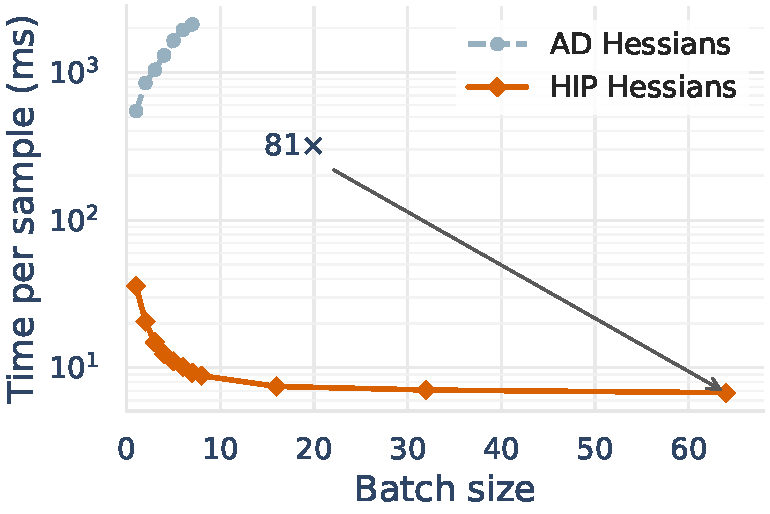
\includegraphics[width=0.5\linewidth]{plots/time_batching.png}
    \caption{\textbf{Compute scaling of HIP compared to AD.} We are measuring the time per sample it takes for increasingly larger batch size. While HIP becomes faster per sample as it efficiently parallelizes, AD becomes slower.}
    \label{fig:batch_timing}
\end{figure}
We observe rapid degradation in the AD Hessian speed with increasing batch size. To explain this, we have to understand exactly how AD treats Hessians. From the point of view of the AD engine, there is no difference between a batch of two molecules of system size $N_A$ and $N_B$, and a larger system of size $N_A + N_B$. In both cases, the MLIP function takes in an array of dimension $3N_A + 3N_B$, and returns either a single scalar $E_A + E_B$ or even worse, an array $[E_A, E_B]$, so mathematically the energy function looks like $E(\mathbf{R}): \mathbb{R}^{3N_A + 3N_B} \rightarrow \mathbb{R}$ or $E(\mathbf{R}): \mathbb{R}^{3N_A + 3N_B} \rightarrow \mathbb{R}^2$. Consequently, a Hessian of this function is a block diagonal matrix of dimension $3(N_A + N_B) \times 3(N_A + N_B)$, or even $2\times 3(N_A + N_B) \times 3(N_A + N_B)$. Therefore, the memory costs grow quadratically with the batch size. Since we have to implement the Hessian calculation using sequential Hessian-Vector products to avoid running out of memory, we cannot even take advantage of parallelization in batched Hessian processing.




\subsection{Additional results}
\begin{figure}
    \centering
    \includegraphics[width=0.99\linewidth]{plots/hessian_heatmap_idx12345.png}
    \caption{\textbf{HIP compared to ground-truth DFT Hessian.} The horizontal and vertical axis index the $(3N_{Atoms})^2$ entries of the Hessian. We depict the absolute values of test sample C5H6O in eV/\AA$^2$.}
    \label{fig:hessian_heatmap}
\end{figure}

\subsubsection{Loss function\label{sec:lossablation}}
We are trying to design a loss function that emphasizes the lowest lying eigenvalues/eigenvectors.
To design such a loss function, one could naively compute a loss directly as $L= \sum_i^k |\mathbf{v}_i^\text{predict} - \mathbf{v}_1^\text{true}|$. This requires computing the eigenvalues and eigenvectors of the true and predicted Hessian via an eigenspectrum decomposition. Unfortunately, backpropagation through such an eigenspectrum decomposition is numerically unstable \citep{aaComputationEigenvalueEigenvector2007}.
First, gradients computed using the eigenvectors tensor will only be finite when $\mathbf{H}$ has distinct eigenvalues. Furthermore, if the distance between any two eigenvalues is close to zero, the gradient will be highly sensitive, as it depends on the eigenvalues $\lambda_i $ through the computation of
$
\min_{i \neq j} \frac{1}{\lambda_i - \lambda_j}
$.
Instead, we propose the following subspace loss.

In the following section, we compare the eigenspace loss that we introduced in \eqref{eq:eigenloss} to the standard choice of mean square error (MSE) and mean absolute error (MAE). 

In particular, we emphasize the subspace $k=8$. This is because transition state search, ZPE, and frequency analysis for extrema classification all depend on the two lowest-lying eigenvectors and eigenvalues. We choose $k=8$ instead of $k=2$ to account for the usual $6$ redundant degrees of freedom, which we do not remove during training for numerical stability.

We combine the subspace loss with MAE, so the total loss becomes
\begin{align}
    \mathcal{L}_\text{MAE+Sub} 
    &= \mathcal{L}_\text{MAE} + \mathcal{L}_\text{sub}^{(k=8)} \\
    &=
    \sum_{i,j} |\mathbf{H}_{i,j} - \mathbf{H}^\text{pred}_{i,j}|
     + \sum_{i,j} \left|\mathbf{V}_{[:,:k]}^\top \mathbf{H}^\text{pred}\mathbf{V}_{[:,:8]} - \mathbf{\Lambda}_{[:,:8]}\right|_{i,j} 
     % + \gamma \sum_{i,j} \left|\mathbf{V}_{[:,k:]}^\top \mathbf{H}^\text{pred}\mathbf{V}_{[:,k:]} - \mathbf{\Lambda}_{[:,k:]}\right|_{i,j}
\end{align}
For simplicity, we weight both the MAE and subspace loss equally. Future work could benefit from carefully tuning the relative weights between the loss terms.

On downstream tasks, subspace loss improves over MAE and MSE in (i) transition state search, as shown in Table \ref{tab:loss_tssearch}, and (ii) transition state identification frequency analysis, as shown in Table \ref{tab:loss_freqanalysis}. We observe equal performance between MAE and the subspace loss for (i) geometry relaxation Table \ref{fig:loss_relax} and (ii) computing the zero-point energy Table \ref{tab:loss_zpe}.

Table \ref{tab:loss_acc} shows that the subspace loss improves the first eigenvector $\bm{v}_1$ cosine similarity, and the second eigenvalue $\lambda_2$ MAE. This is consistent with the better performance of the subspace loss on transition state-related tasks, since the transition state is characterized via the two smallest eigenvalues $\lambda_1, \lambda_2$, and is found by following the first eigenvector $\bm{v}_1$.

MSE generally underperforms compared to MAE and MAE with subspace loss.
MSE has the theoretical advantage of being rotation-invariant, whereas MAE is not.
In practice, however, we find that the MSE leads to a high variance (spikes) in the training loss and gradient norm across batches. We speculate that MAE outperforms MSE due to training stability.

Hessian prediction with any loss function tested significantly outperforms prior AD Hessians.

% Accuracy
\begin{table}
\centering
\resizebox{0.99\textwidth}{!}{
\centering
% \begin{tabular}{llccccc}
% \hline
% \multirow{2}{*}{Loss} & \multirow{2}{*}{Model} & Hessian $\downarrow$  & Eigenvalues $\downarrow$ & CosSim $\bm{v}_1$ $\uparrow$ & $\lambda_1$ $\downarrow$ & Time $\downarrow$ 
%  & & eV/\AA$^2$ & eV/\AA$^2$ & unitless & eV/\AA$^2$ & ms 
% \hline
% MSE & EquiformerV2 & 0.033 & 0.072 & 0.728 & 0.168 & 38.7 
% MAE & EquiformerV2 & \textbf{ 0.026 } & \textbf{ 0.057 } & 0.825 & \textbf{ 0.127 } & 38.6 
% MAE+Sub & EquiformerV2 & 0.030 & 0.063 & \textbf{ 0.870 } & 0.130 & 38.5 
\begin{tabular}{lccccccccc}
\hline
\multirow{2}{*}{Loss}  & Hessian $\downarrow$  & Eigenvalues $\downarrow$ & CosSim $\bm{v}_1$ $\uparrow$ & $\lambda_1$ $\downarrow$ & $\lambda_2$ $\downarrow$ & $\lambda_1^{E}$ $\downarrow$ & $\lambda_2^{E}$ $\downarrow$ & CosSim $\bm{v}_1^{E}$ $\uparrow$ & CosSim $\bm{v}_2^{E}$ $\uparrow$ \\
 & eV/\AA$^2$ & eV/\AA$^2$ & unitless & eV/\AA$^2$ & eV/\AA$^2$ & eV/\AA$^2$ & eV/\AA$^2$ & unitless & unitless \\
\hline
MSE  & 0.033 & 0.072 & 0.728 & 0.168 & 0.088 & 0.037 & 0.013 & 0.959 & 0.928\\
MAE  & \textbf{ 0.026 } & \textbf{ 0.057 } & 0.825 & \textbf{ 0.127 } & 0.052 & \textbf{ 0.031 } & 0.012 & 0.976 & 0.952 \\
MAE+Sub  & 0.030 & 0.063 & \textbf{ 0.870 } & 0.130 & \textbf{ 0.030 } & 0.031 & \textbf{ 0.010 } & \textbf{ 0.980 } & \textbf{ 0.957 } \\
\hline
\end{tabular}
}
\caption{Accuracy of HIP-EquiformerV2 using different loss functions. Superscript $E$ denotes after removing redundant degrees of freedom using Eckart-projection on the mass-weighted matrix.}
\label{tab:loss_acc}
\end{table}

% Second order optimization
\begin{figure}
    \centering
    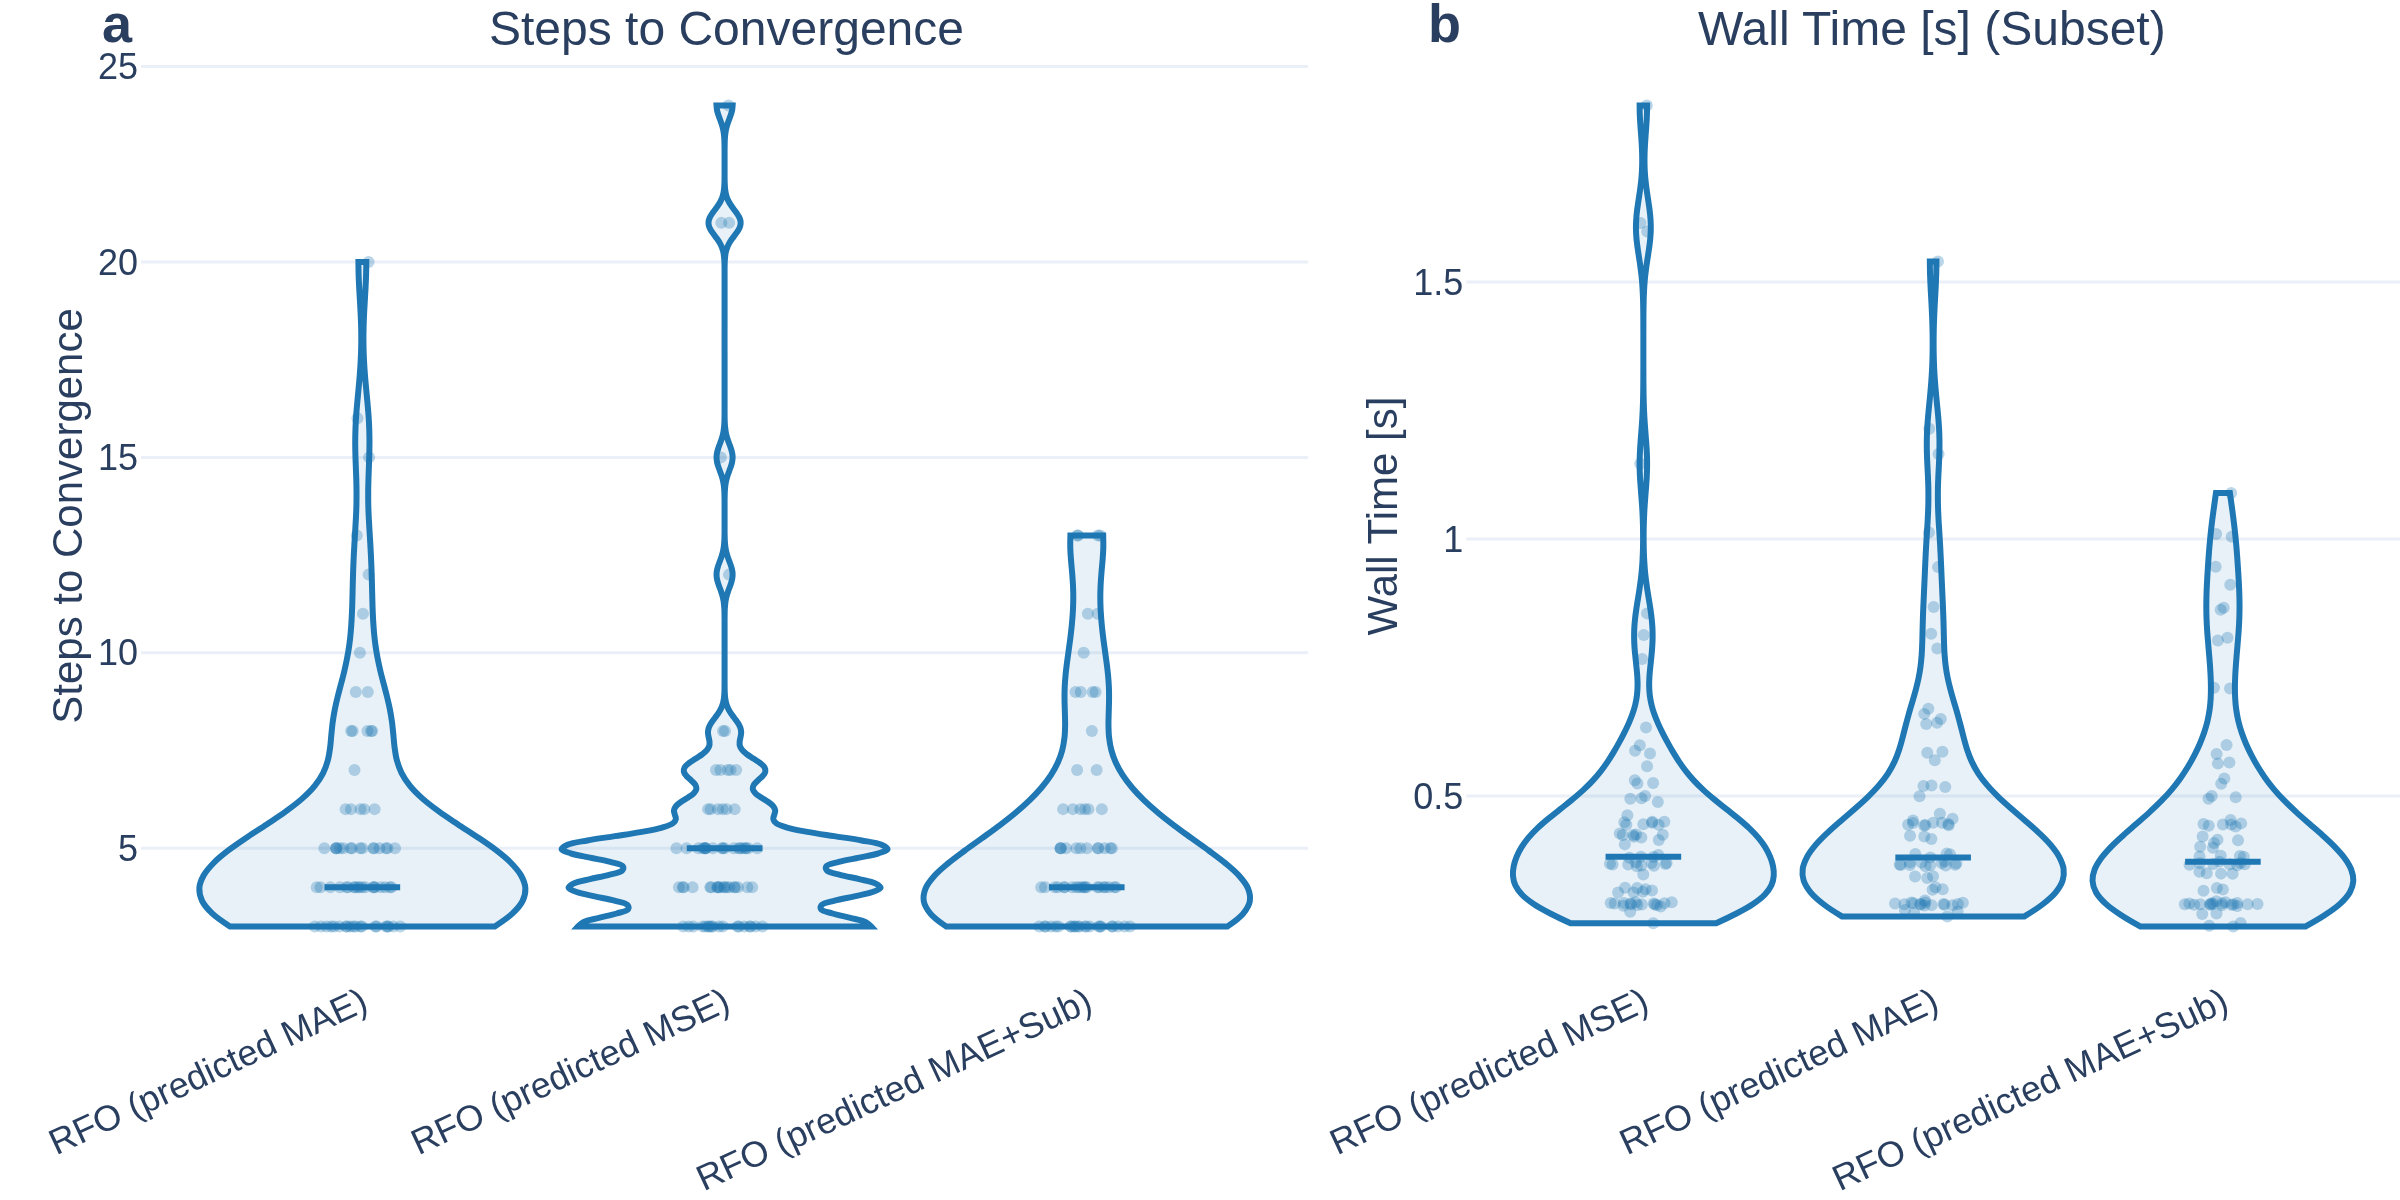
\includegraphics[width=0.75\linewidth]{plots/relaxations_lossablation.png}
    \caption{Geometry relaxation with HIP-EquiformerV2 trained using different loss functions}
    \label{fig:loss_relax}
\end{figure}

\begin{table}
\centering
\resizebox{0.7\textwidth}{!}{
\centering
\begin{tabular}{llll}
\toprule
Hessian & Model & ZPE MAE (Std) [eV] & $\Delta$ZPE MAE (Std) [eV] \\
\midrule
MSE & HIP-EquiformerV2 & 0.0008 (0.0012) & 0.0019 (0.0025) \\
MAE & HIP-EquiformerV2 & 0.0004 (0.0004) & \textbf{0.0013 (0.0019)} \\
MAE+Sub & HIP-EquiformerV2 & \textbf{0.0004 (0.0003)} & 0.0016 (0.0018) \\
\bottomrule
\end{tabular}
}
\caption{Zero-point energy by HIP-EquiformerV2 for different loss functions}
\label{tab:loss_zpe}
\end{table}

% TS search
\begin{table}
\centering
\resizebox{0.6\textwidth}{!}{
\centering
\begin{tabular}{llcccc}
\hline
Loss & Model & TS Success & RFO Converged & Both \\
\hline
MSE & HIP-EquiformerV2 & 718 & 669 & 659 \\
MAE & HIP-EquiformerV2 & 740 & 693 & 683 \\
MAE+Sub & HIP-EquiformerV2 & \textbf{750} & \textbf{705} & \textbf{698} \\
\hline
\end{tabular}
}
\caption{Transition state search with HIP-EquiformerV2 trained with different loss functions}
\label{tab:loss_tssearch}
\end{table}

\begin{table}
\centering
\resizebox{0.75\textwidth}{!}{
\centering
\begin{tabular}{lccccccc}
\hline
Name & TPR $\uparrow$ & FPR $\downarrow$ & FNR $\downarrow$ & TNR $\uparrow$ & Precision $\uparrow$ & Accuracy $\uparrow$&  Accuracy All $\uparrow$ \\
\hline
MSE  & 88\% & 11\%  & 12\%  & 89\% & 86\% & 89\% & 86\% \\
MAE  & 93\% & 7\%  & 7\%  & 93\% & 91\% & 93\% & 91\%  \\
MAE+Sub  & \textbf{93\%} & \textbf{6\%}  & \textbf{7\%}  & \textbf{94\%} & \textbf{92\%} & \textbf{94\%} & \textbf{92\%} \\
\hline
\end{tabular}
}
\caption{Identifying transition states (left) and any extrema (rightmost column) via frequency analysis using HIP-EquiformerV2 for different loss functions.}
\label{tab:loss_freqanalysis}
\end{table}



% \subsubsection{Computational cost compared to finite difference}
% \begin{figure}
%     \centering
%     \includegraphics[width=0.8\linewidth]{plots/speed_memory_finitedifference.png}
%     \caption{
%     \textbf{Computational cost.} Comparing (a) time and (b) memory of a forward without Hessians, with HIP, automatic differentiation (AD), finite difference Hessians. The memory for Forward Pass, FD Hessians, and HIP Hessians is nearly identical.
%     }
%     \label{fig:speedmemoryfinitedifference}
% \end{figure}
% \cite{wander2025accessing} showed that finite-difference Hessians obtained from finetuned MLIPs can increase success rates in transition state search for catalysis. The advantage of finite difference is that it does not require additional memory over a regular forward pass, and only force labels are needed for training. The limitation of finite-difference Hessians is their high computational cost. Like AD Hessians, finite difference requires $O(N^2)$ time, but with an even larger prefactor, as can be seen in Fig. \ref{fig:speedmemoryfinitedifference}.





\subsection{Experimental Details}

\subsubsection{Training}

The hyperparameters of our HIP-EquiformerV2 model are listed in \ref{tab:hyperparameters}. We inherit the model settings and large parts of the optimizer settings from the HORM codebase \citep{cui2025horm}.

\begin{table}[h]
\centering
\resizebox{0.65\textwidth}{!}{ % Resize to fit the page width
\begin{tabular}{ll}
\hline
% \textbf{Category} & \textbf{Hyperparameter (Value)} 
\hline
Model & Type: EquiformerV2 \\
      & Layers: 4 \\
      & Sphere channels: 128 \\
      & Attention hidden channels: 64 \\
      & Attention heads: 4 \\
      & Attention alpha channels: 64 \\
      & Attention value channels: 64 \\
      & FFN hidden channels: 128 \\
      & Activation: SiLU \\
      & Distance basis: 512 (Gaussian) \\
      & Radius cutoff: 12 Angstrom \\
      & Cutoff Hessian: 12 Angstrom \\
      & Hessian layers: 3 (1 for end-to-end) \\
      & Spherical harmonics: Lmax=4, Mmax=2 \\
      & Grid resolution: 18, Sphere samples: 128 \\
      & Dropout: $\alpha$=0, drop path=0 \\
\hline
Loss & MAE weight: 1 \\
     & Eigen subspace $k$: 8 \\
     & Eigen loss weight $\alpha$: 1.0 \\
\hline
Optimizer & AdamW \\
          & Betas: (0.9, 0.999) \\
          & AMSGrad: True \\
          & Weight decay: 0 \\
        & Batch size: 128 \\
         & Gradient clipping: 0.1 (norm) \\
\hline
Learning Rate 
          & Learning rate: 0.0005 \\
        & Scheduler: StepLR \\
          & Step size: 10 \\
          & Gamma: 0.85 \\
Trainer & Steps: 500k (3-5 days on a H100 GPU) \\
\hline
\hline
\end{tabular}
} % end resizebox
\caption{\textbf{Hyperparameters}. For simplicity, we use the same hyperparameters for HIP as HORM \citep{cui2025horm}.
}
\label{tab:hyperparameters}
\end{table}

% \paragraph{Training resources\label{sec:trainingresources}}
Training AD Hessians is exceptionally more expensive than training HIP.
The memory cost of computing loss gradients through the full  $3N\times3N$ Hessian is prohibitive. Instead, the baseline models from \cite{cui2025horm} randomly sample one or two columns of the Hessian via random Hessian-vector products at each training step. Despite this, training AD Hessians remains exceedingly expensive. The HORM paper states that they use 2 HVPs at a batch size of 128. Their checkpoint metadata shows a per-device batch size of 8, suggesting a 16$\times$ A30 GPU setup for 1 million gradient steps.
In contrast, we trained HIP on a single H100 GPU for 500k steps. Additionally, each HIP training step costs 1/5 as much as AD Equiformer training on our hardware. Finally, we observe that HIP fully converges after 300-500k training steps, whereas AD Hessians require multiple steps due to the limited supervision and the inability to use the full Hessian.

\begin{table}[h]
\centering
\renewcommand{\arraystretch}{1.6} % Adjust row height
\resizebox{0.8\textwidth}{!}{ % Resize to fit the page width
\begin{tabular}{lccccccc}
\hline
\textbf{Model} & Hessian Columns & Batch Size &
BZ / GPU & GPU & \# GPUs & Training Steps \\
\hline
AlphaNet            & 1 & 32  & 16 & H20 & 2  & 688,000 \\
LeftNet-CF          & 1 & 64  & 16 & A30 & 8  & 192,000 \\
LeftNet-DF          & 2 & 64  & 16 & A30 & 8  & 120,000 \\
EquiformerV2 (E-F)  & 0 & 128 & 8  & A30 & 16 & 384,000 \\
EquiformerV2        & 2 & 128 & 8  & A30 & 16 & 1,008,000 \\
\hline
HIP-EquiformerV2        & 3N (all) & 128 & 128 & H100 & 16 & 500,000 \\
\hline
\end{tabular}
}
\caption{\textbf{Summary of training resources.} Comparing HIP to checkpoints from HORM \citep{cui2025horm}.}
\label{tab:traingpu}
\end{table}

\subsubsection{Geometry Optimization \label{sec:relax_methods}}
We compare our RFO-based optimization \citep{RSRFO1998a} using predicted Hessians (RFO predicted), and our RFO with BFGS updates with initial predicted Hessian (RFO-BFGS predicted init) against first-order methods, quasi-second-order BFGS variants, and exact second-order approaches obtained via automatic differentiation or finite differences. 

Our baselines include steepest descent with backtracking line search (SteepestDescent) and the first-order method FIRE \citep{bitzek2006}. For quasi-second-order methods, we consider RFO with BFGS updates initialized from the identity (RFO-BFGS). For full second-order methods, we include RFO with either automatic differentiation or finite difference Hessians. 
%Namely we report
%(a) steepest descent with backtracking line search (SteepestDescent)
%(b) fast inertial relaxation engine (FIRE) 
%(c) RFO with identity matrix as initial guess, followed by BFGS (RFO-BFGS unit-init)
%(e) RFO+BFGS with learned Hessian as initial guess (RFO-BFGS predicted-init) (ours)
% (f) RFO+BFGS where the Hessian is predicted every third step (RFO-BFGS Hpred-3)
%(f) RFO with predicted Hessian at every step (RFO predicted) (ours)
%(g) RFO+BFGS with AD Hessian as initial guess (RFO-BFGS AD-init)
%(h) RFO with AD Hessian at every step (RFO AD)
%
We run relaxations on 80 reactant geometries from the Transition1x validation set (which is different from HORM-T1x), that we noise with $0.5$ \AA{} RMS. We use the RS-RFO and redundant coordinate implementation in pysisyphus \citep{steinmetzer2021, herbolComputationalImplementationNudged2017}. We set the convergence criteria to "Gaussian default" (see \ref{sec:convergence}), with a budget of 150 steps.

\subsubsection{Transition State Search with ReactBench\label{sec:reactbench}}
We use the recently introduced \href{https://github.com/deepprinciple/ReactBench}{ReactBench} benchmark \citep{zhao2025}, which relies on pysisyphus \citep{steinmetzer2021} and PyGSM\cite{aldazZimmermanGroupPyGSM2025} for implementation of the optimization routines.
The workflow consists of generating an initial guess using the growing string method \citep{aldazZimmermanGroupPyGSM2025, zimmerman2015}, followed by local search using the restricted-step partitioned rational-function-optimization method (RS-P-RFO) \citep{RSRFO1998a}. Finally, convergence to the correct transition state is confirmed by frequency analysis and following the intrinsic reaction coordinate (IRC).
% minimum energy reaction pathway (MERP) in mass-weighted cartesian coordinates between the transition state of a reaction and its reactants and products
Following previous work \citep{zhao2025, cui2025horm}, we report success metrics of each step: 
\begin{enumerate}
    \item 
GSM successfully converged below a force RMS of $5e^{-5}$ Hartree/Bohr within 100 iterations ("GSM Success")
\item After RS-P-RFO, the frequency analysis determines geometry as a true transition state ("TS Success")
\item IRC converged to the same criteria and yields the original initial reactant and product ("IRC Verified").
\end{enumerate}
We then treat the samples successfully passing (a)-(c) as transition state proposals, and verify for a random subset of 100, if the DFT Hessians have one negative eigenvalue and the DFT force RMS is below $2e^{-3}$ Ha/Bohr. We additionally report if RS-P-RFO converged to "Gaussian default" (\ref{sec:convergence}) within 50 steps.

\subsubsection{Zero-Point Energy\label{sec:zpe_setup}}
Starting from 80 reactant and product geometries from the Transition1x validation set, we relax the geometries using DFT and RS-RFO (BFGS, identity initialization) until "Gaussian tight" convergence (see \ref{sec:convergence}).
For a given method $m$, the reaction ZPE change is
$$
\Delta \mathrm{ZPE}_{m}
= \mathrm{ZPE}_{m}(\text{product}) - \mathrm{ZPE}_{m}(\text{reactant}).
$$
The $\Delta\Delta$DFT error for a model is
$$
\Delta\Delta \mathrm{ZPE}
= \bigl|\Delta \mathrm{ZPE}_{\text{model}} - \Delta \mathrm{ZPE}_{\text{DFT}}\bigr|.
$$
We use the same level of theory for model relaxation as for model training.
Then we compute the ZPE from the Eckart-projected, mass-weighted Hessian, as predicted by the different models, and compare it to DFT.
We report all energies in eV per molecule. 

\subsubsection{Convergence Criteria\label{sec:convergence}}
Throughout our experiments, we adopt the following convergence criteria, as shown in table \ref{tab:convergence_criteria}, set forth by the Gaussian software and widely used across different codebases.
All criteria need to be met for a geometry to be considered converged.

\begin{table}
\centering
\resizebox{0.75\textwidth}{!}{
\centering
\begin{tabular}{lccccc}
\toprule
Setting & Max Force & RMS Force & Max Step & RMS Step & Used for \\
\midrule
% Gaussian loose             & 1.7e-3 & 1.0e-2 & 6.7e-3 & &  \\
Gaussian default           & 4.5e-4 & 3.0e-4 & 1.8e-3 & 1.2e-3 & Relaxation, TS search \ref{sec:relax} \\
Gaussian tight             & 1.5e-5 & 1.0e-5  & 6.0e-5 & 4.0e-5 & ZPE \ref{sec:zpe} \\
% Gaussian very tight        & 1.0e-6 &         & 6.0e-6 & 4.0e-6 & 
\bottomrule
\end{tabular}
}
\caption{Convergence criteria used in our experiments}
\label{tab:convergence_criteria}
\end{table}



\subsubsection{Glycine proton transfer\label{sec:glycinedetails}}

To assess whether the predicted Hessians encode physically meaningful curvature near a transition state, we selected a reaction for which the relevant chemical motion can be described by simple internal coordinates. We first annotated all non-training reactions in Transition1x by comparing reactant and product bond graphs, excluding the training split and considering both the validation and test splits. For each reaction, we recorded the bonds formed and broken, the number of connected molecular components, and a coarse reaction-family label. We then prioritized reactions with a small number of bond changes and an unambiguous two-dimensional representation of the reaction coordinate.

We chose the intramolecular proton transfer of glycine, present in the Transition1x test split (sample ID 5, rxn1961). Glycine is the simplest amino acid, and its neutral-zwitterionic tautomerization,
\(
\mathrm{NH_2CH_2COOH \rightleftharpoons NH_3^+CH_2COO^-},
\)
has been widely studied as a model proton-transfer process. In this reaction, the acidic carboxyl proton is transferred between an oxygen and the amine nitrogen, interconverting O--H- and N--H-bonded forms. The transferring proton is therefore naturally described by the two distances
\(
q_{\mathrm{NH}} = d(\mathrm{N4},\mathrm{H9}), \qquad
q_{\mathrm{OH}} = d(\mathrm{O3},\mathrm{H9}).
\)
Previous studies of glycine tautomerization have commonly used a proton-transfer coordinate based on these distances
\(\xi = q_{\mathrm{NH}} - q_{\mathrm{OH}}\) (see e.g. \cite{zhang2024glycine}). 

% \paragraph{2D collective variables}
% Here, we instead use a two-dimensional coordinate system consisting of the antisymmetric proton-transfer coordinate
% \[
% s = q_{\mathrm{NH}} - q_{\mathrm{OH}}
% \]
% and the symmetric compression coordinate
% \[
% \sigma = q_{\mathrm{NH}} + q_{\mathrm{OH}}.
% \]
% This representation separates progress along the proton-transfer coordinate from changes in the total N--H/O--H distance and provides a compact visualization of the local potential-energy surface around the transition state.

We first investigate a two-dimensional surface around the proton transfer.
For each point on the 
% \((\xi,\sigma)\) 
\((q_{\mathrm{NH}}, q_{\mathrm{OH}})\)
surface, we constructed an initial geometry by starting from the Transition1x \citep{schreiner2022transition1x} transition-state structure and placing the transferring proton to satisfy the target values of \(q_{\mathrm{NH}}\) and \(q_{\mathrm{OH}}\). We excluded any pair \((q_{\mathrm{NH}}, q_{\mathrm{OH}})\) that violated the triangle inequality
\(
q_{\mathrm{NH}} + q_{\mathrm{OH}} < d(\mathrm{N4},\mathrm{O3})
\quad \mathrm{or} \quad
|q_{\mathrm{NH}} - q_{\mathrm{OH}}| > d(\mathrm{N4},\mathrm{O3}).
\)
The remaining structures were relaxed while constraining \(q_{\mathrm{NH}}\) and \(q_{\mathrm{OH}}\), allowing all other degrees of freedom to relax. 
They were first relaxed with GFN2-xTB, using TBLite and ASE BFGS.
% from ase.constraints import FixInternals
% from ase.optimize import BFGS
% from tblite.ase import TBLite
% atoms.set_constraint(FixInternals(bonds=[[q_nh, [N_ATOM, H_ATOM]], [q_oh, [O_ATOM, H_ATOM]]]))
% atoms.calc = TBLite(method="GFN2-xTB", verbosity=0)
% opt = BFGS(atoms, logfile=None)
% opt.run(fmax=0.05, steps=300)
They were then reoptimized at the DFT level using ORCA 6.1.1 with
\texttt{! wB97X-D3 6-31G(d) TightSCF Opt}.
The remaining structures were first relaxed with fixed \(q_{\mathrm{NH}}\) and \(q_{\mathrm{OH}}\), allowing all other degrees of freedom to relax, and were then reoptimized at the DFT level with the same two bond-distance constraints. This produced 579 DFT-relaxed geometries.

For each DFT-relaxed geometry, we computed energies, forces, and Hessians using ORCA 6.1.1 \cite{ORCA} with the \(\omega\)B97X-D3 functional and the 6-31G(d) basis set. Geometry optimizations used
\texttt{! wB97X-D3 6-31G(d) TightSCF Opt}
with the two proton-transfer bond distances constrained. Energies and forces were then evaluated with
\texttt{! wB97X-D3 6-31G(d) TightSCF EnGrad},
and Hessians were evaluated with
\texttt{! wB97X-D3 6-31G(d) TightSCF Freq}.
The data is available at \url{huggingface.co/andreasburger/hip/tree/main/orca_wb97x_d3_631gd_glycine_pt_dft_relaxed_579}.
The resulting energy surface is shown in figure~\ref{fig:glycine_forcefield}.
\begin{figure}
    \centering
    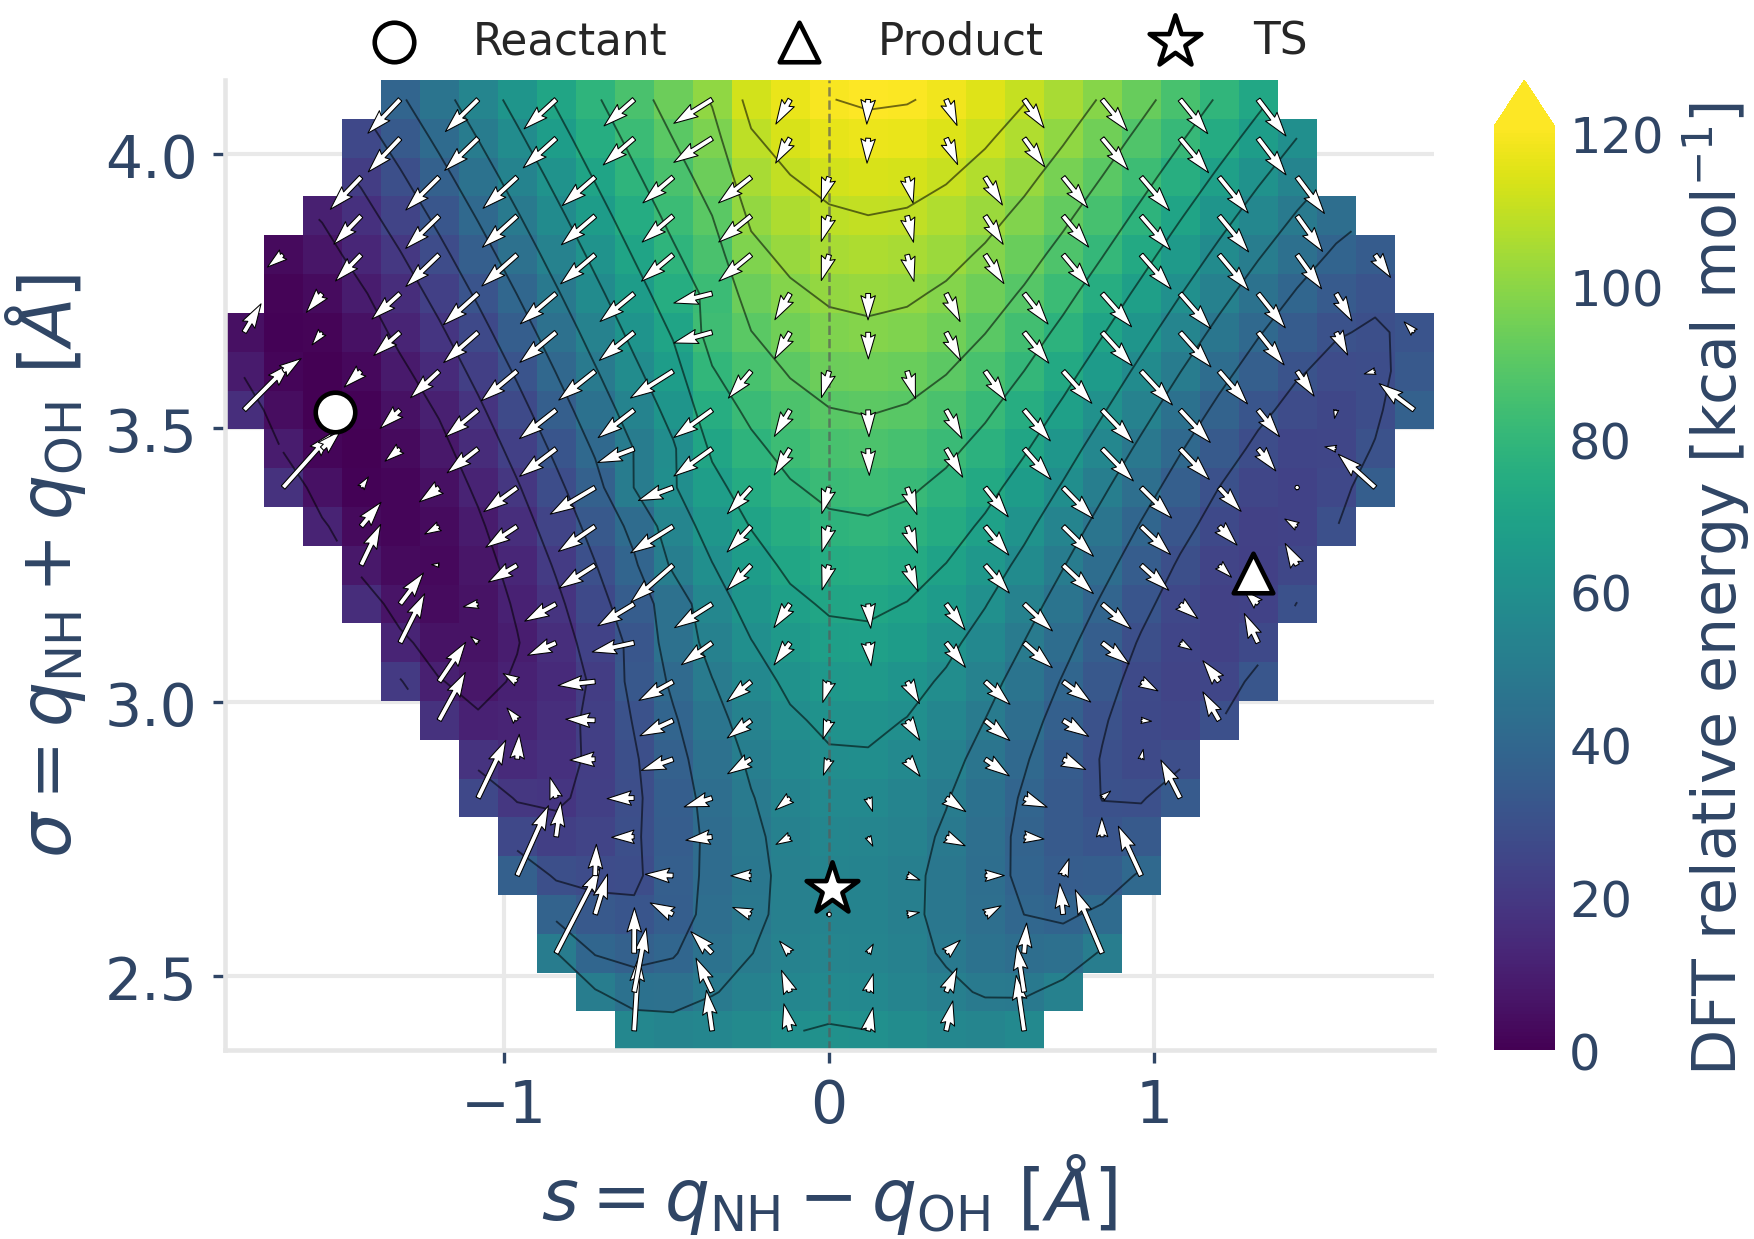
\includegraphics[width=0.52\linewidth]{plots/glycine_dftrelaxed_forcefield.png}
    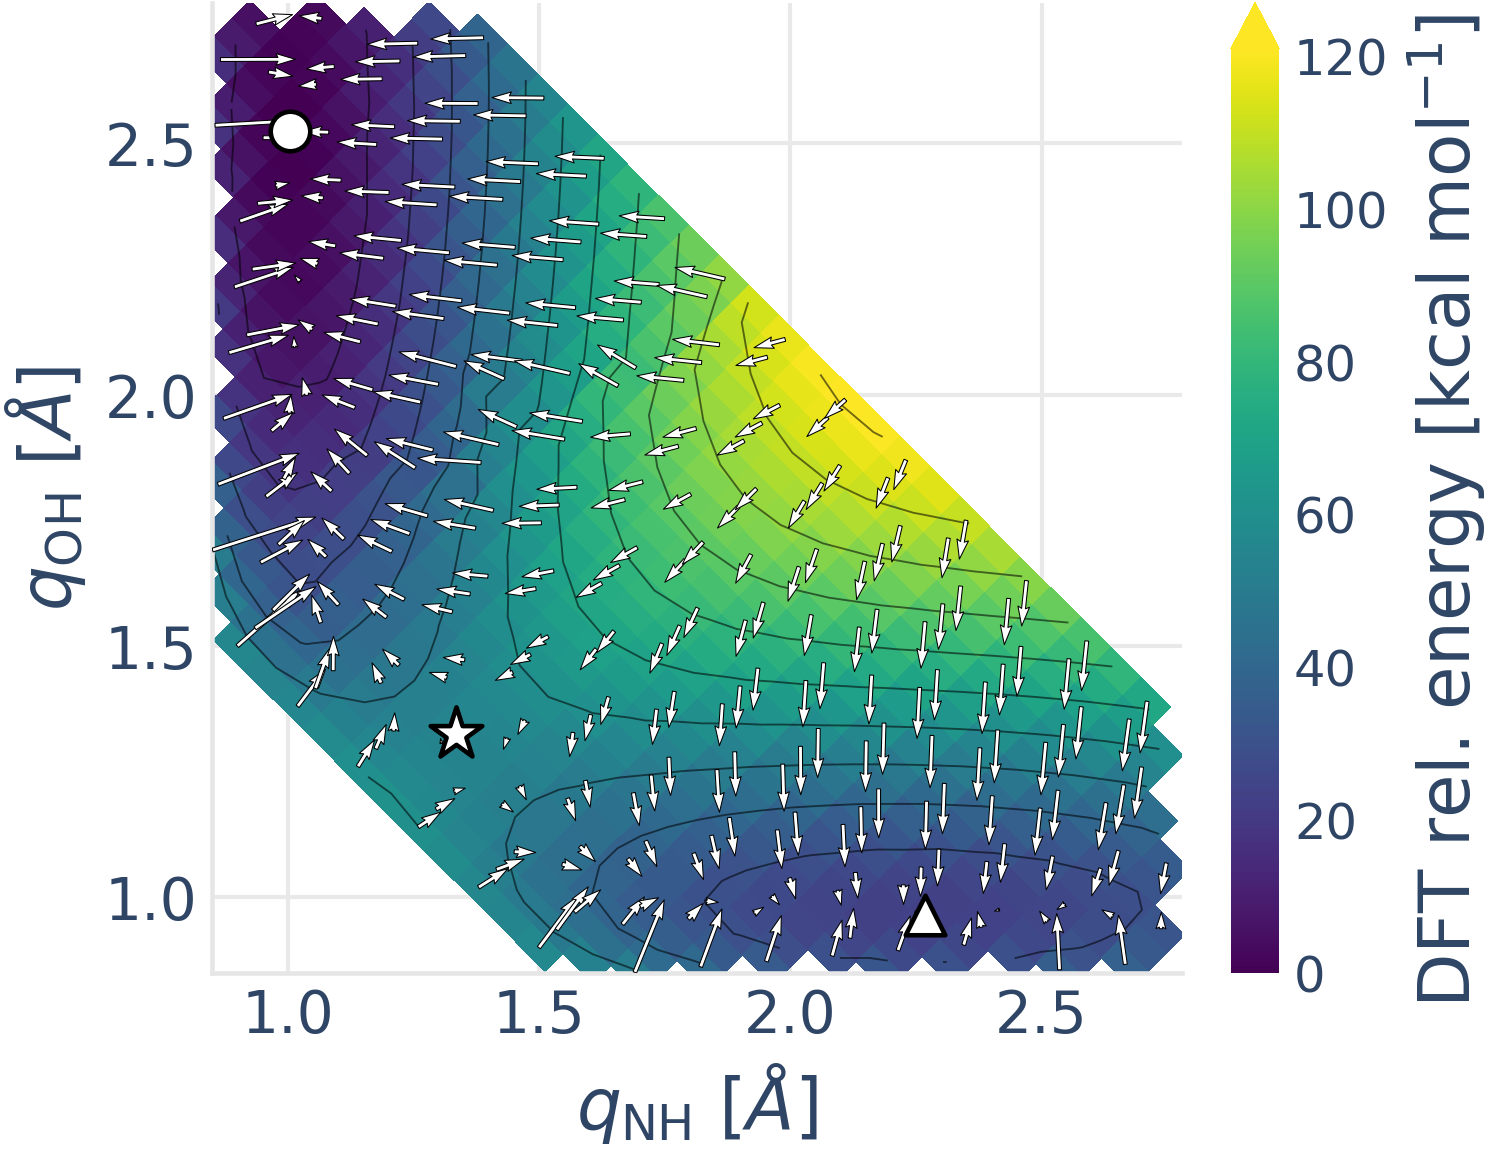
\includegraphics[width=0.45\linewidth]{plots/glycine_dftrelaxed_forcefield_q.png}
     \caption{
     \textbf{Glycine.} 
     2D collective variable energy surface at $\omega$B97X/6-31G(d), with forces shown as arrows. 
     % The star marks the transition state. The top right corner corresponds to the hydrogen dissociating from the molecule.
     The DFT-optimized reactant and product contain no imaginary frequencies, while the DFT transition-state optimization yields one imaginary frequency, confirming the expected minimum/first-order-saddle classifications.
     }
     \label{fig:glycine_forcefield}
\end{figure}

% \paragraph{1D minimum energy path}
We also study the one-dimensional minimum energy path for the same glycine proton-transfer reaction to evaluate model behaviour along a chemically meaningful trajectory. We used the stored Transition1x record, which contains 266 geometries, which we interpreted as an initial 10-image NEB path followed by 32 saved blocks of 8 internal NEB/CINEB images. We used the final saved block of 8 with the reactant and product geometries as the 10-image minimum energy path.

To obtain a smooth trajectory for evaluation and visualization, we connected adjacent images along this path using geodesic interpolation in redundant internal-coordinate space. The original NEB images were kept fixed. This produced 150 path geometries. All methods were evaluated on the same fixed structures. Again, single-point energies, forces, and Cartesian Hessians were computed for each geometry using ORCA 6.1.1 with \texttt{! wB97X-D3 6-31G(d) TightSCF EnGrad Freq} and are available at \url{huggingface.co/andreasburger/hip/tree/main/orca_wb97x_631gd_glycine_mep_145}.


\subsubsection{Size generalization on PubChem\label{sec:pubchemorca}}

To test Hessian prediction beyond the HORM training distribution, we assembled a benchmark of 710 neutral organic molecules containing only C, H, N, and O, with 30–100 atoms (71 atom-count bins, 10 molecules per bin). Geometries were drawn from the PubChem database via the PUG REST API. For each target atom count \(N\), we enumerated stoichiometrically plausible neutral CHNO formulas and queried PubChem for matching compounds (`fastformula` endpoint, up to 12 CIDs per formula). Candidates were retained only if they satisfied 
(a) formal charge 0 (PubChem `Charge` property)
(b) composition restricted to \(\{Z=1,6,7,8\}\) (c) exactly \(N\) atoms in the 3D structure.

We first attempted to retrieve PubChem 3D conformers (SDF). When no suitable 3D structure was available, we generated a conformer from the isomeric SMILES using RDKit (ETKDGv3 embedding followed by MMFF or UFF relaxation). Uncovered atom-count bins were additionally filled from deterministic RDKit-generated CHNO conformers. 
Reference energies, Cartesian gradients, and Hessians were computed with ORCA~6
at $\omega$B97X/6-31G(d), \texttt{TightSCF}, on the fixed input geometries
(charge~$0$, multiplicity~$1$).
We used two single-point jobs per molecule:
(i)~a \texttt{Freq} calculation for the analytical Hessian, and
(ii)~an \texttt{EnGrad} calculation for the energy and gradient.
\begin{verbatim}
! wB97X 6-31G(d) TightSCF Freq
! wB97X 6-31G(d) TightSCF EnGrad
%pal nprocs 8 end
%maxcore 4000
\end{verbatim}
The reference dataset and geometries are released under \url{huggingface.co/andreasburger/hip/tree/main/orca_wb97x_631gd_chno_30_100}.

For aggregate PubChem plots, we remove pathological molecules before bin-wise averaging.
Outliers are identified from the per-molecule Cartesian Hessian MAE,
\(
  \mathrm{MAE}(\mathbf{H}) = \frac{1}{9N^2}\sum_{i,j=1}^{3N}\left|H^{\mathrm{pred}}_{ij}-H^{\mathrm{ref}}_{ij}\right|,
\)
where $N$ is the number of atoms.
For each atom-count bin $N$, let $\{x_i\}_{i=1}^{n_N}$ denote the Hessian MAEs of molecules in that bin, with $n_N=10$.
We compute the bin median $\tilde{x}_N$ and the median absolute deviation
\(
  \mathrm{MAD}_N = \operatorname{median}_i\!\left(\left|x_i-\tilde{x}_N\right|\right).
\)
The modified $z$-score of sample $i$ is
\(
  M_i = 0.6745\,\frac{x_i-\tilde{x}_N}{\mathrm{MAD}_N},
\)
following Iglewicz and Hoaglin \citep{iglewicz1993outliers}. This modified $z$-score uses the median instead of the mean, and MAD instead of the variance, to improve robustness. The prefactor $0.6745$ is the median absolute deviation of a standard normal variable.
Sample $i$ is flagged as an outlier if it exceeds $|M_i|>10$.
Outliers are detected independently for each method, and the union of flagged
samples is removed from all methods so that curves remain comparable.
This removes 10 of 710 PubChem molecules.

Because raw Cartesian Hessian eigenvalues mix internal and external (translation/rotation) modes, we additionally project both reference and predicted Hessians onto the vibrational subspace using Eckart projection (mass-weighted, translation–rotation removal) and compare the resulting eigenvalue spectra. The eigenvalue MAE is computed as
\(
\mathrm{MAE}_\lambda = \langle |\lambda^{\mathrm{pred}}_k - \lambda^{\mathrm{ref}}_k| \rangle,
\)
where \(\{\lambda_k\}\) are the projected vibrational eigenvalues $eV/Ų$. 
% We also report agreement on the number of imaginary modes (negative eigenvalues after projection).


\end{appendices}

%%===========================================================================================%%
%% If you are submitting to one of the Nature Portfolio journals, using the eJP submission   %%
%% system, please include the references within the manuscript file itself. You may do this  %%
%% by copying the reference list from your .bbl file, paste it into the main manuscript .tex %%
%% file, and delete the associated \verb+\bibliography+ commands.                            %%
%%===========================================================================================%%



\end{document}
